% APA 7th Edition manuscript with BSDS capstone front matter
\documentclass[man, 12pt, letterpaper, floatsintext]{apa7}

% --- Encoding & Fonts ---
\usepackage[utf8]{inputenc}
\usepackage[T1]{fontenc}
\usepackage{times}
% Reset monospace to CM Typewriter (Courier oblique not in basic TeX Live)
\renewcommand{\ttdefault}{cmtt}

% --- Packages ---
\usepackage{graphicx}
\usepackage{amsmath}
\usepackage{array}
\usepackage{booktabs}
\usepackage{calc}
\usepackage{longtable}
\usepackage{tikz}
\usetikzlibrary{shapes.geometric, arrows.meta, positioning}
% Flush-left (ragged-right) fixed-width column type for tables, to match the APA flush-left body
\newcolumntype{L}[1]{>{\raggedright\arraybackslash}p{#1}}
\geometry{left=1.5in,right=1in,top=1in,bottom=1in}

\providecommand{\tightlist}{%
    \setlength{\itemsep}{0pt}\setlength{\parskip}{0pt}}
\newcounter{none}
\renewcommand{\thenone}{}
\providecommand*{\theHnone}{\arabic{none}}
\setlength{\parindent}{0.5in}
\setlength{\parskip}{0pt}

% --- Bibliography (APA 7 via biblatex) ---
\usepackage[style=apa, backend=biber]{biblatex}
\addbibresource{biblio.bib}

% --- Title Page Metadata ---
\title{Predicting Residential Property Values in Metro Cebu Using Machine Learning with GIS-Derived Spatial Features}
\shorttitle{Metro Cebu Property Valuation}
\authorsnames{Chris Dominic Estreba}
\authorsaffiliations{University of Asia and the Pacific}

\begin{document}

\pagenumbering{roman}
\setcounter{page}{1}

% Title page. Deliberately NOT the LaTeX `titlepage` environment: that
% environment resets the page counter to 1 at its end, which made the approval
% sheet repeat page "i". Setting the page manually keeps the count running so the
% title page is i and the approval sheet is ii. Page number is suppressed here
% (\thispagestyle{empty}) but the page is still counted.
\thispagestyle{empty}
\phantomsection
\addcontentsline{toc}{section}{Title}
% Single-space the title page (the class double-spaces the body); this also keeps
% the page from spilling onto a second sheet, which would push the approval sheet
% off page ii.
{\linespread{1}\selectfont
\begin{center}
\vspace*{1.0in}

{\bfseries Predicting Open-Market Residential Property Values in Metro Cebu Using Machine Learning and Geospatial Features\par}

\vspace{1.25in}

Presented to the

\vspace{0.25in}

Faculty of the Data Science Program

Department of Mathematics

School of Sciences, Engineering, and Technology

University of Asia and the Pacific

\vspace{0.75in}

In Partial Fulfillment of the

Requirements for the Degree of

Bachelor of Science in Data Science

\vspace{0.9in}

By

\vspace{0.25in}

Chris Dominic Estreba

\vspace{0.75in}

June 2026
\end{center}
\par}
\clearpage

\clearpage
\section*{Approval Sheet}
\addcontentsline{toc}{section}{Approval Sheet}

The capstone entitled Predicting Open-Market Residential Property Values in Metro Cebu Using Machine Learning and Geospatial Features, prepared and submitted by \textbf{Chris Dominic Estreba} in partial fulfillment of the requirements of the degree of Bachelor of Science in Data Science, is approved.

\vspace{.5in}

\noindent\textbf{Ms. Kimberly May M. Vallesteros}\\
Faculty in-charge\\
School of Sciences and Engineering\\
University of Asia and the Pacific

\vspace{0.3in}

PANEL

\vspace{0.5in}

\noindent\textbf{Mr. Randy Marasigan}\\
Capstone Adviser

\vspace{0.5in}

\noindent\textbf{Ms. Kimberly May M. Vallesteros}\\
Panelist

\vspace{0.5in}

\noindent\textbf{Mr. Elmer Peramo}\\
Panelist

% \clearpage
\section*{Dedication}
\addcontentsline{toc}{section}{Dedication}

This page is reserved for the dedication.
  % Dedication is optional; removed per APA 7 capstone format
\clearpage
\section*{Abstract}
\addcontentsline{toc}{section}{Abstract}

This study developed a residential property valuation framework for Metro Cebu using machine learning and GIS-derived spatial features. The work addressed the gap between administrative benchmarks, lender-driven appraisals, and market-facing price signals by assembling a hybrid dataset of residential properties from institutional acquired assets, foreclosure listings, and open-market online listings. The study focused on six local government units in Metro Cebu: Cebu City, Mandaue City, Lapu-Lapu City, Talisay City, Minglanilla, and Consolacion.

The methodology combined structural, locational, administrative, and geospatial variables. Property records were geocoded, matched with barangay-level BIR zonal values, and enriched with accessibility and neighborhood-context features, including proximity to major economic nodes, amenity access, and a neighborhood price lag. Because property types are priced on very different per-square-meter logics, separate models were fitted for condominiums, houses, and vacant lots, on a price-per-square-meter target. Within each stratum, three predictive approaches were compared: hedonic regression, Random Forest, and XGBoost. Under leak-free grouped cross-validation, the tree-based models outperformed the hedonic baseline, while Random Forest and XGBoost performed comparably; Random Forest was deployed in all three strata for its robustness on small samples and its simpler implementation. The deployed models reached a typical error of about 19, 23, and 38 percent (median absolute percentage error) for condominiums, houses, and vacant lots, with location features carrying most of the predictive signal. Model outputs were interpreted through SHAP-based explainability and prepared for use through a QGIS map and a web-based decision-support application centered on a predicted residential price surface.

The manuscript positions the study as a predictive and prescriptive tool for residential valuation practice in Metro Cebu. Its contribution lies in combining property-level machine learning, spatial feature engineering, and transparent explanation into a locally grounded decision-support framework that is more responsive to urban change than static administrative benchmarks alone.

\clearpage
\section*{Acknowledgment}
\addcontentsline{toc}{section}{Acknowledgment}

% DRAFT — adjust wording, titles, and ordering to your own voice as needed.

I would like to express my sincere gratitude to the people who made this capstone possible.

To my adviser, Mr. Randy Marasigan, thank you for keeping me pointed toward the goal whenever I lost sight of it.

To my panel, Ms. Kimberly May M. Vallesteros and Mr. Elmer Peramo, thank you for the questions and feedback that sharpened both the method and the argument. I am grateful as well to Ms. Vallesteros, faculty in-charge, for her support throughout the program.

To my professors in the School of Sciences, Engineering, and Technology --- Sir Vince Cruz, Sir Durwin Santos, Sir Ken Liberanza, Dr. Noemi Torre, Ms. Mili Singson, Sir Michael Sanchez, and Dr. Edwin Olmos --- and to the many others I have not named here who were no less instrumental, thank you for the instruction and formation that shaped me as a student at the University of Asia and the Pacific.

To my parents, Falconerie Estreba and Sigmund Estreba, and my sister, Marielle Estreba, thank you for supporting me through this milestone in my studies. Even from home, your prayers and encouragement carried me through.

To my classmates and friends --- Josh, Mica, Dante, Marcus, Trish, Kurt, Yana, Keefe, and El --- thank you for the company, the laughs, and the memories we made along the way.

Above all, I thank God for the guidance and strength that carried me through this journey. There were many days when I had little left of my own, and I still made it through. I am grateful for that.


\clearpage
\phantomsection
\addcontentsline{toc}{section}{Table of Contents}
\tableofcontents

\clearpage
\phantomsection
\addcontentsline{toc}{section}{List of Tables}
\listoftables

\clearpage
\phantomsection
\addcontentsline{toc}{section}{List of Figures}
\listoffigures

\clearpage
\phantomsection
\addcontentsline{toc}{section}{List of Maps}
\listof{ccmap}{List of Maps}

\clearpage
\section*{List of Pictures}
\addcontentsline{toc}{section}{List of Pictures}

No pictures have been listed yet.

% No \clearpage: let the List of Appendices follow the List of Pictures on the same page.
\vspace{0.45in}
\phantomsection
\addcontentsline{toc}{section}{List of Appendices}
\section*{List of Appendices}

\begingroup
\setlength{\parindent}{0pt}
\noindent\makebox[1.05in][l]{Appendix~\ref{app:datadoc}}Data Documentation\dotfill\pageref{app:datadoc}\par
\noindent\makebox[1.05in][l]{Appendix~\ref{app:portals}}Data Source Portals\dotfill\pageref{app:portals}\par
\noindent\makebox[1.05in][l]{Appendix~\ref{app:supptables}}Supplementary Tables\dotfill\pageref{app:supptables}\par
\noindent\makebox[1.05in][l]{Appendix~\ref{app:shap}}SHAP Beeswarm Plots\dotfill\pageref{app:shap}\par
\noindent\makebox[1.05in][l]{Appendix~\ref{app:snapshots}}Feature Snapshots by Stratum\dotfill\pageref{app:snapshots}\par
\noindent\makebox[1.05in][l]{Appendix~\ref{app:olsdiag}}OLS Diagnostic Plots\dotfill\pageref{app:olsdiag}\par
\noindent\makebox[1.05in][l]{Appendix~\ref{app:webapp}}Web Application Screenshots\dotfill\pageref{app:webapp}\par
\endgroup

\clearpage
\section*{List of Abbreviations and Acronyms}
\addcontentsline{toc}{section}{List of Abbreviations and Acronyms}

\begin{longtable}{p{0.20\textwidth} p{0.68\textwidth}}
ABT & Analytics Base Table \\
APA & American Psychological Association \\
BIR & Bureau of Internal Revenue \\
BSP & Bangko Sentral ng Pilipinas \\
CBD & Central Business District \\
CBRT & Cebu Bus Rapid Transit \\
CRISP-DM & Cross-Industry Standard Process for Data Mining \\
GIS & Geographic Information System \\
IVS & International Valuation Standards \\
LGU & Local Government Unit \\
MCRAI & Metro Cebu Residential Accessibility Index \\
OLS & Ordinary Least Squares \\
OSM & OpenStreetMap \\
POI & Point of Interest \\
ROPA & Real and Other Properties Acquired \\
RPPI & Residential Real Estate Price Index \\
SHAP & SHapley Additive exPlanations \\
\end{longtable}


\clearpage
\pagenumbering{arabic}
\setcounter{page}{1}

\section{Introduction}\label{introduction}

\subsection{\texorpdfstring{\textbf{Background of the Study}}{Background of the Study}}\label{background-of-the-study}

\subsubsection{\texorpdfstring{\textbf{What is Real Estate?}}{What is Real Estate?}}\label{what-is-real-estate}

Real estate sits at the intersection of shelter, commerce, and investment. Under Article 415 of the Philippine Civil Code, immovable property includes land, buildings, and permanent attachments. Unlike many other assets, real estate is both something people use and something they price, finance, and trade.

In actual transactions, that price is shaped by several actors with different interests. Brokers and agents facilitate sales, banks finance purchases and assess collateral risk, appraisers estimate value, and local government units set administrative benchmarks such as zonal values for taxation. Although these actors approach property from different functions, all depend on a defensible estimate of value. This study examined how that value is determined, how fair it is, and how transparent the valuation process can be.

\subsubsection{\texorpdfstring{\textbf{Real Estate in Cebu}}{Real Estate in Cebu}}\label{real-estate-in-cebu}

Cebu has become one of the Philippines' most dynamic regional economies, recording 7.3\% growth in 2024 (PSA Region 7, 2025). Much of this growth has come from the IT-BPM sector, the expansion of call center activity, and the post-pandemic recovery of tourism, hospitality, and retail. These shifts have fed directly into demand for residential and mixed-use property.

Across Metro Cebu, particularly Cebu City, Mandaue, Lapu-Lapu, Talisay, Minglanilla, and Consolacion, that demand has made the property market notably active. Residential property prices in the area rose by 11.5\% in 2025, the highest rate outside the National Capital Region (BSP, 2025).

That pressure is also being reinforced by infrastructure projects that are changing accessibility across the urban area. The Cebu Bus Rapid Transit (CBRT), the Metro Cebu Expressway, and the continued development of the South Road Properties are likely to affect land values by altering connectivity, travel times, and the attractiveness of nearby locations. For a valuation study, these spatial shifts matter because they change not only where demand is strongest, but also how quickly existing benchmarks can become outdated.

\subsubsection{\texorpdfstring{\textbf{The Problem: How is Price Decided in Cebu?}}{The Problem: How is Price Decided in Cebu?}}\label{the-problem-how-is-price-decided-in-cebu}

Despite this growth, the property pricing system in Metro Cebu is still assembled from several partial and often inconsistent reference points. In practice, three sources are used most often, and each has clear limitations.

First, BIR zonal values serve as administrative benchmarks for taxation, but they often lag behind actual market conditions. A 2023 appraisal review found that only 60\% of LGUs nationwide had updated their assessment schedules (Otsuka et al., 2023), which suggests that some zonal values in Cebu may no longer reflect current prices. Second, bank appraisals are designed mainly to manage lending risk, so they may produce values that are more conservative than open-market prices. Third, listing prices and agent quotes often reflect asking positions rather than verified transaction values, and these are not standardized across platforms or sellers.

The result is a valuation gap between official benchmarks, estimates based on lenders, and prices that markets are seemingly willing to bear. For buyers and sellers, this makes pricing harder to interpret. For banks, it complicates collateral assessment. For local governments, it weakens the connection between tax benchmarks and market reality. Metro Cebu therefore has an active property market, but not yet a consistent and validated valuation system at the property level.

\subsubsection{\texorpdfstring{\textbf{Why Metro Cebu, and Why Now?}}{Why Metro Cebu, and Why Now?}}\label{why-metro-cebu-and-why-now}

Three converging factors make it timely to build a data-driven valuation model for Metro Cebu:

\begin{enumerate}
\item \textbf{Prices are moving faster than the benchmarks can follow}: With 11.5\% growth in 2025 and some zonal values outdated since 2019, the gap between official benchmarks and market reality is widening. Continued reliance on outdated models perpetuates mispricing.
\item \textbf{Infrastructure is redrawing the value map in real time}: Projects like the CBRT and the Expressway are restructuring barangay accessibility and desirability. Traditional appraisal methods, reliant on historical comparables, cannot price these spatial changes in real time. A GIS-augmented model built on geocoded property data addresses this constraint.
\item \textbf{The data now exists to do this properly}: Online platforms such as Lamudi, open geospatial data, and geocoding tools (Google Maps API) enable the construction of a property-level dataset without requiring private deed-of-sale records. Open-source GIS software also allows us to transform this data into an interactive web map, providing prescriptive spatial decision support for practitioners.
\end{enumerate}

\subsubsection{\texorpdfstring{\textbf{Ideal Scenario}}{Ideal Scenario}}\label{ideal-scenario}

The core problem is not that Cebu lacks valuation activity, but that the activity still lacks a common, evidence-based basis. A data-driven model that quantifies the contribution of specific value drivers, such as lot area, proximity to economic nodes, nearby amenities, and neighborhood trends, would provide reproducible estimates for residential properties. Delivered through an interactive QGIS map and a Streamlit web application, this model would help move Cebu from heuristic pricing toward a more transparent and evidence-based valuation process aligned with IVS 2025.

\begin{center}\rule{0.5\linewidth}{0.5pt}\end{center}

\subsection{\texorpdfstring{\textbf{Statement of the Problem}}{Statement of the Problem}}\label{statement-of-the-problem}

\textbf{Decision Problem}: How can real estate firms in Metro Cebu utilize data-driven models, augmented with geospatial feature engineering, to predict property values more accurately and consistently?

\textbf{Research Problem}: In Metro Cebu, reliance on outdated administrative benchmarks and manual appraisals produces inconsistent, subjective pricing. No existing study combines property-level data with GIS-derived geospatial features (network distance, MCRAI scoring, spatial autocorrelation) for the Metro Cebu market, and none provides a spatial decision-support layer for valuation practice.

\begin{center}\rule{0.5\linewidth}{0.5pt}\end{center}

\subsection{\texorpdfstring{\textbf{Research Questions}}{Research Questions}}\label{research-questions}

\begin{enumerate}
\item What value drivers significantly influence property prices in Metro Cebu?
\item Which modeling technique---\textbf{Hedonic Regression}, \textbf{Random Forest}, or \textbf{XGBoost}---produces the most accurate valuation out of sample (lowest MAPE)?
\item Do \textbf{geospatial features}---proximity to economic nodes, MCRAI accessibility measures, and spatial autocorrelation---significantly improve model performance compared to structural-only models?
\item How large is the ``Valuation Gap'' between the model's data-driven predictions and traditional BIR Zonal Values?
\end{enumerate}

\begin{center}\rule{0.5\linewidth}{0.5pt}\end{center}

\subsection{\texorpdfstring{\textbf{Significance of the Study}}{Significance of the Study}}\label{significance-of-the-study}

Addressing this valuation gap benefits multiple stakeholders:

\begin{enumerate}
\item \textbf{Real Estate Brokers and Appraisers}: Provides standardized tools compliant with IVS 2025 transparency requirements, including SHAP-based explainability, an interactive QGIS map for spatial analysis, and a Streamlit interface for property-level valuation review.
\item \textbf{Property Investors}: Ensures fair, data-backed pricing and helps identify undervalued areas visually through geospatial heatmaps.
\item \textbf{Banks and Lending Institutions}: Improves collateral assessment accuracy through reproducible, auditable models, which reduce exposure to pricing errors that manual appraisals can miss.
\item \textbf{Local Government Units (LGUs)}: Facilitates the updating of zonal values using market-based evidence, mapping the geographic divergence between official and actual prices.
\end{enumerate}

This study is significant within the Philippine context as the first Cebu-specific, data-driven valuation model integrating GIS-based feature engineering. While prior Philippine machine learning studies focus on Metro Manila or use aggregate indices, no work applies geocoded network-distance features, MCRAI scoring, and spatial autocorrelation to property-level data for Metro Cebu. By delivering results through QGIS-ready map layers and a Streamlit web application, the study extends predictive analytics into applied decision support for a fragmented local market.

\begin{center}\rule{0.5\linewidth}{0.5pt}\end{center}

\subsection{\texorpdfstring{\textbf{Scope and Limitations}}{Scope and Limitations}}\label{scope-and-limitations}

\subsubsection{\texorpdfstring{\textbf{Scope}}{Scope}}\label{scope}

This study focuses on the residential real estate market within Metro Cebu. While the National Economic and Development Authority (NEDA) defines Metro Cebu as encompassing 13 LGUs, this study operationally scopes ``Metro Cebu'' to its central urban core: \textbf{Cebu City, Mandaue, Lapu-Lapu, Talisay, Minglanilla, and Consolacion}. This constraint ensures high data density and robust geospatial analysis, as these six LGUs represent the most active transaction zones and the highest concentration of infrastructure development. Figure~\ref{fig:study-area} shows the spatial extent of this scope and the locations of the eight polycentric CBD nodes used in the model.

\begin{figure}[htbp]
\centering
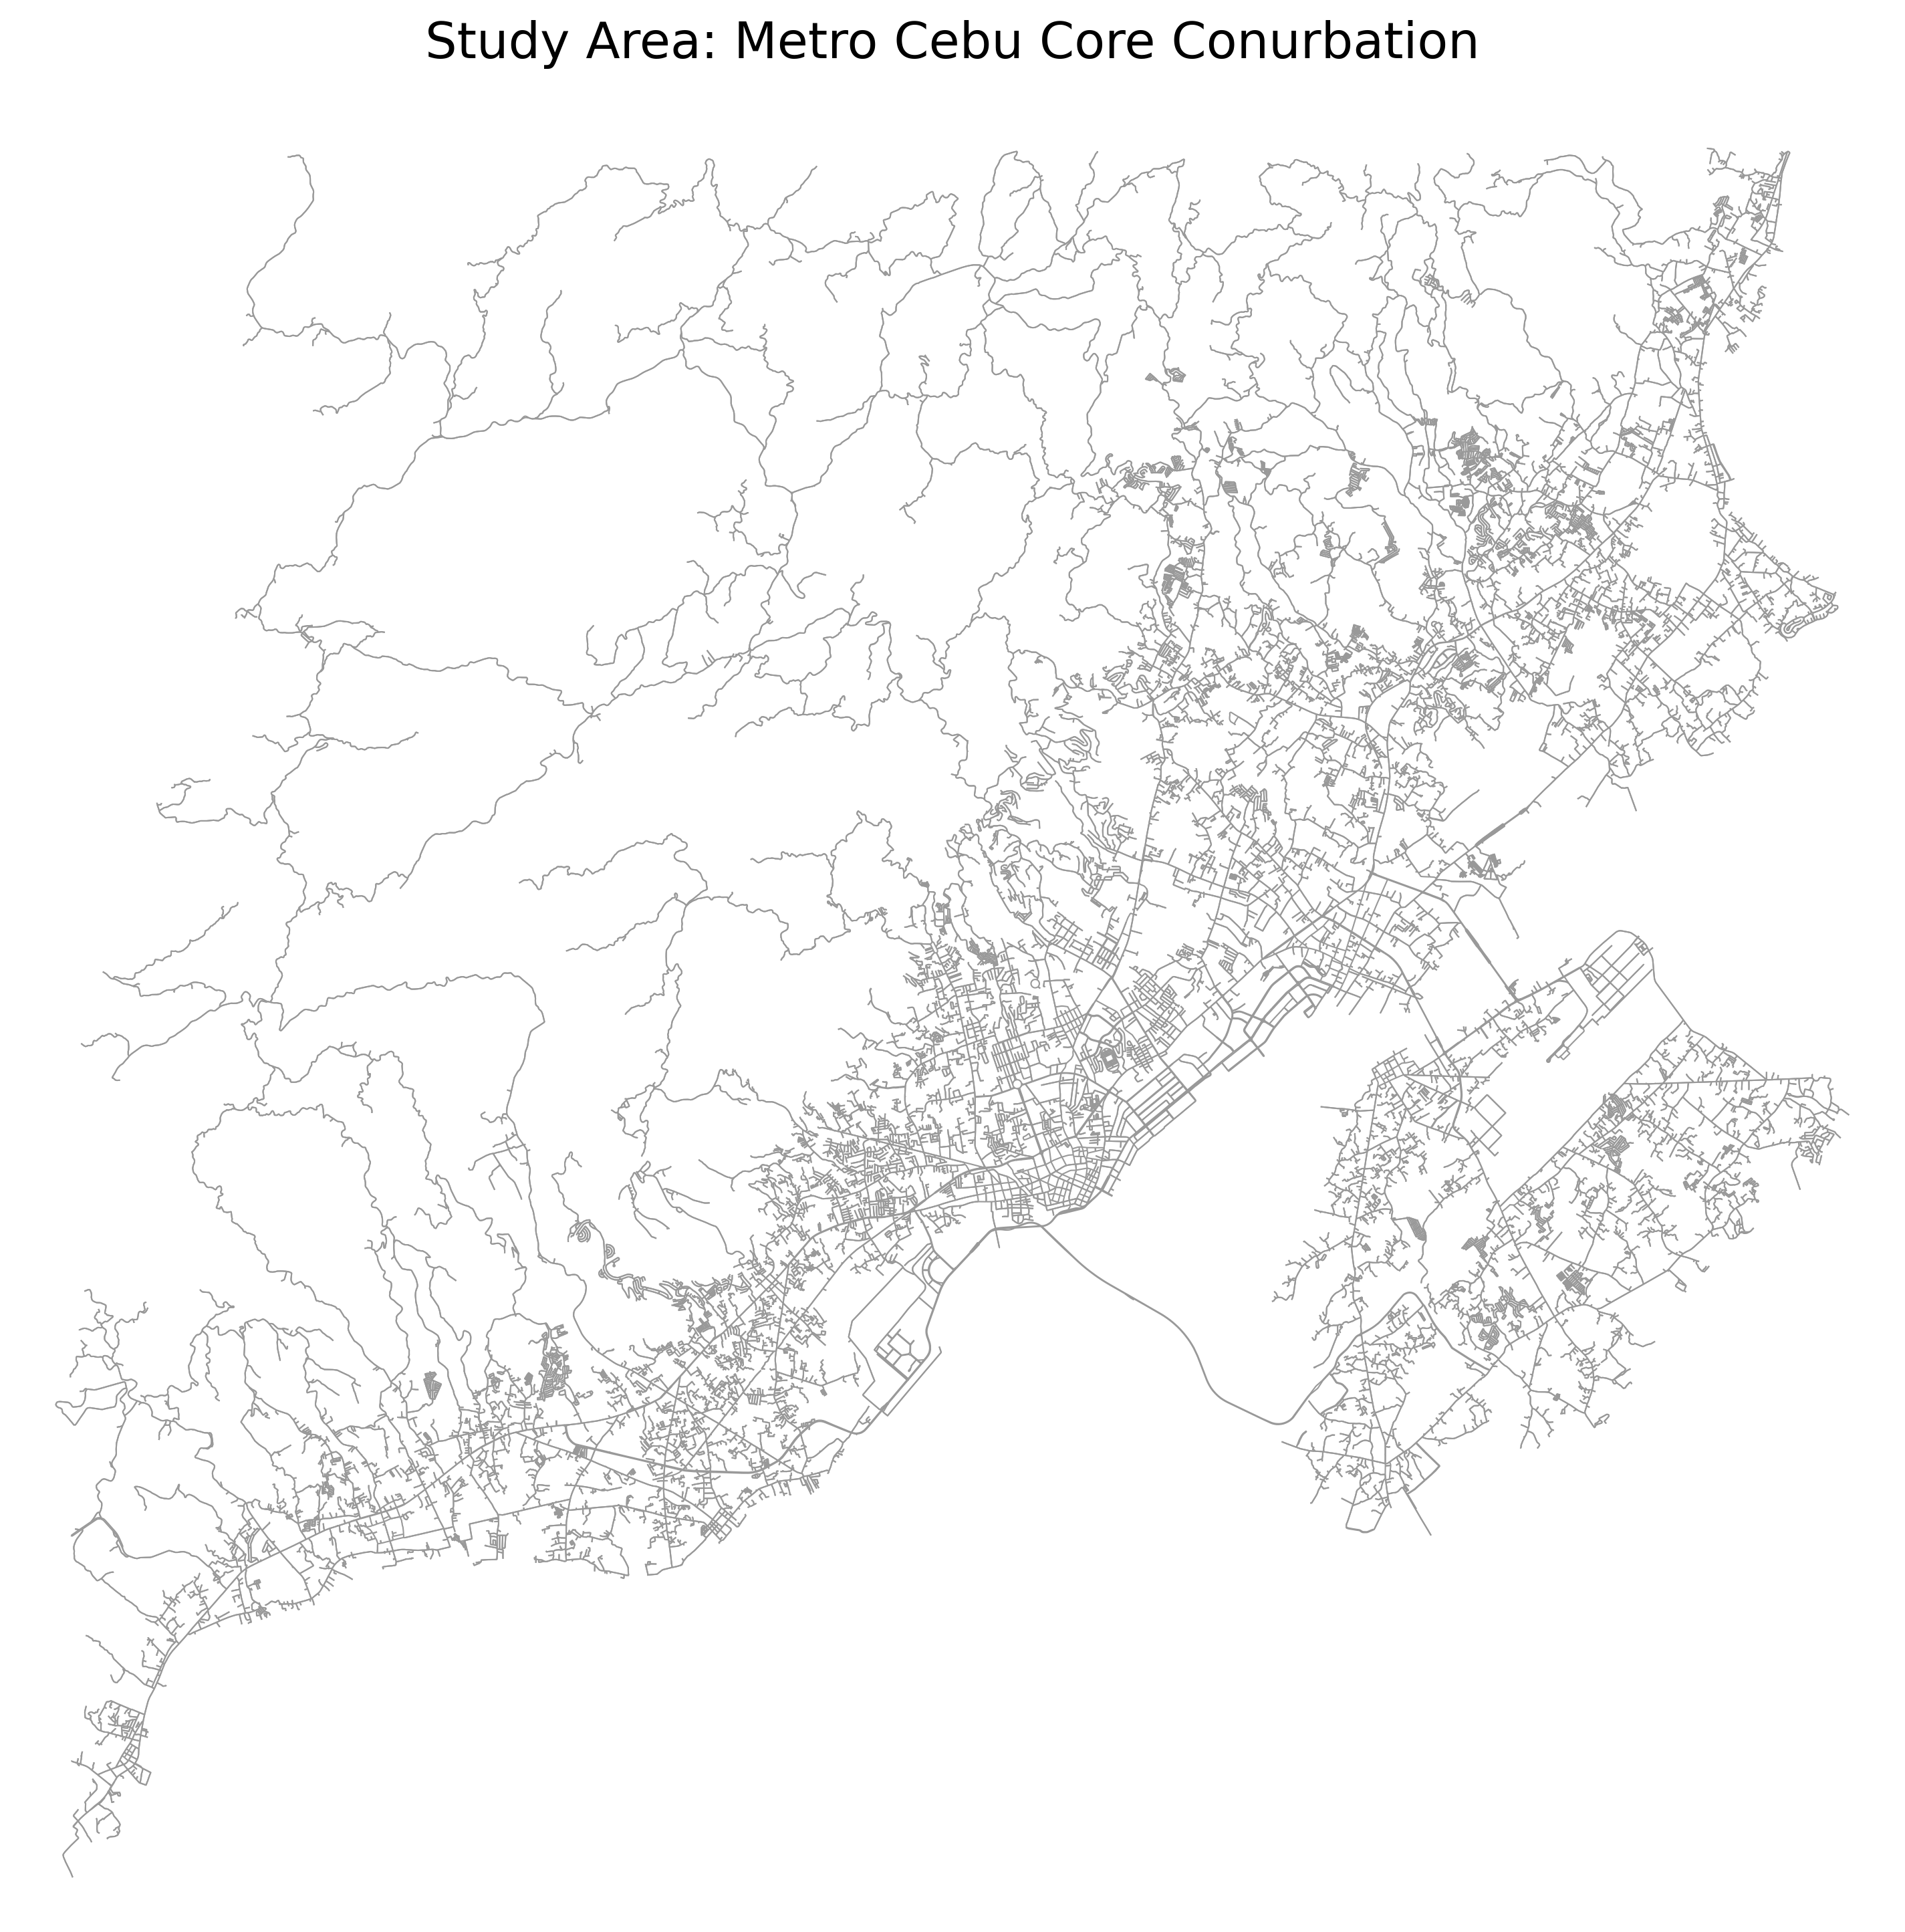
\includegraphics[width=0.90\textwidth]{diagrams/Study-Area-Map.png}
\caption{Metro Cebu Study Area. The six LGUs in the study scope are shown alongside the eight polycentric CBD nodes used for network-distance feature engineering: Cebu Business Park, Mandaue CBD, Mactan CBD, South Road Properties, Talisay Tabunok, Consolacion, Naga City (anchor only), and Mactan-Cebu International Airport.}
\label{fig:study-area}
\end{figure}

The primary data sources include:

The study drew on six data sources covering open-market listings, bank foreclosure records, administrative floor-price benchmarks, BIR zonal values, geospatial APIs, and road network data. Each source is described in detail in Chapter 3, Section 3.2.

The study evaluated three predictive models: \textbf{Hedonic Regression (OLS)}, \textbf{Random Forest}, and \textbf{XGBoost} (see Section 1.6 for rationale). Geospatial features were engineered through geocoding, road-network distance, MCRAI scoring, and spatial lag computation. The canonical ABT preserved the wider market evidence base, but the final fitted model was restricted to the \emph{open\_market} segment so that the deployed output stayed aligned with a market-value use case.

The study produced two applied deliverables: QGIS-ready spatial layers for valuation review and a Streamlit web application combining an open-market residential price surface with property-level prediction and explanation.

\subsubsection{\texorpdfstring{\textbf{Limitations}}{Limitations}}\label{limitations}

\begin{enumerate}
\item \textbf{Open-Market Listing Bias}: The deployed model was fitted on open-market listings rather than verified deed-of-sale transactions. This kept the prediction target aligned with market-facing pricing, but it also meant that seller strategy and asking-price noise remained in the data.
\item \textbf{Unobserved Heterogeneity}: The model cannot capture qualitative features omitted from listings, such as interior finish quality or views, typically assessed during physical inspections.
\item \textbf{Geospatial Approximation}: Addresses are geocoded via Google Maps API, which may introduce minor spatial errors compared to exact lot-parcel shapefiles. Additionally, OSM coverage in peripheral barangays may be less robust than in the urban core.
\item \textbf{Temporal Scope}: The analysis provides a cross-sectional snapshot as of late 2025; it does not capture long-term cyclical real estate trends.
\item \textbf{Geographic Coverage}: The six selected LGUs represent the urban conurbation but exclude the broader municipalities of Cebu Province.
\end{enumerate}

\begin{center}\rule{0.5\linewidth}{0.5pt}\end{center}

\subsection{\texorpdfstring{\textbf{Model Selection Rationale}}{Model Selection Rationale}}\label{model-selection-rationale}

This study employs three complementary models that span the interpretability--accuracy spectrum. This trio has been validated in comparable emerging-market real estate studies \parencite{yacim2018,pai2020}.

\begin{itemize}
\item \textbf{Hedonic Regression (OLS)} serves as the interpretable baseline. It is the established standard in property valuation \parencite{rosen1974}, embedded in both the Philippine Valuation Standards (PVS, 2018) and IVS 2025. OLS produces explicit coefficients for each value driver, directly quantifying their price contribution. We extend it with a spatial lag term to account for autocorrelation among neighboring properties.
\item \textbf{Random Forest} \parencite{breiman2001} addresses the linearity assumption of OLS by capturing non-linear interactions between value drivers---particularly relevant for Metro Cebu housing data, where structural and locational effects are unlikely to remain linear. Its bagging mechanism also provides robustness against outliers.
\item \textbf{XGBoost} \parencite{chen2016} was included as a strong candidate for predictive accuracy: gradient boosting consistently performs well on structured tabular data \parencite{grinsztajn2022} and integrates natively with SHAP \parencite{lundberg2017} to provide property-level explainability, a practical requirement under IVS 2025 transparency standards. The final evaluation in Chapter 7 determines which model best meets the deployment criteria.
\end{itemize}

\subsubsection{\texorpdfstring{\textbf{Why Not Other Models?}}{Why Not Other Models?}}\label{why-not-other-models}

Several alternatives were evaluated but ultimately set aside:

\begin{table}[htbp]
\caption{Models Considered but Not Retained in the Study Design}
\label{tab:chapter1-model-exclusions}
\begin{center}
\begin{tabular}{p{0.23\textwidth} p{0.63\textwidth}}
\toprule
Model & Rationale for Exclusion \\
\midrule
Deep Neural Networks & Require \textgreater{}10,000 labeled samples; our dataset size is insufficient, and global interpretability is sacrificed. \\
Support Vector Regression & Computationally expensive to tune; poor native interpretability; generally weaker than boosting on tabular data. \\
LASSO / Ridge & Constrained by linearity assumptions; effectively subsumed by the OLS baseline for our purposes. \\
\bottomrule
\end{tabular}
\end{center}
\end{table}

\begin{center}\rule{0.5\linewidth}{0.5pt}\end{center}

\section{Review of Related Literature}\label{review-of-related-literature}

\subsection{\texorpdfstring{\textbf{Purpose}}{Purpose}}\label{purpose}

This chapter reviews the existing body of knowledge on data-driven property valuation, drawing from both Philippine and international literature. It establishes the theoretical foundations underpinning this study, surveys empirical evidence on machine learning approaches to real estate pricing, and identifies a critical research gap: the absence of a Cebu-specific, property-level, ML-augmented valuation model.

The review moves from valuation concepts and the Philippine setting to the practical constraints that shape valuation work in emerging markets. It then turns to modeling approaches, the use of geospatial features in property valuation, macroeconomic influences, and the compliance issues that matter if these models are to be used in practice. The chapter closes by identifying the specific gap that this study addresses in the Metro Cebu context.

\begin{center}\rule{0.5\linewidth}{0.5pt}\end{center}

\subsection{\texorpdfstring{\textbf{Core Concepts and Philippine Context}}{Core Concepts and Philippine Context}}\label{core-concepts-and-philippine-context}

\subsubsection{\texorpdfstring{\textbf{Valuation Foundations}}{Valuation Foundations}}\label{valuation-foundations}

Market value is the most probable price under fair, open-market conditions on the valuation date. Market price is the amount actually paid in a specific transaction; the two can differ in practice \parencite{pvs2018}. Hedonic Pricing Theory, introduced by \textcite{rosen1974}, provides the foundational framework for this study. It posits that the price of a differentiated good---such as a house---can be decomposed into a function of its constituent attributes: $P = f(\text{Structural}, \text{Locational}, \text{Environmental})$. This theory underpins the hedonic regression model used as our interpretive baseline.

\subsubsection{\texorpdfstring{\textbf{Philippine Indices and Administrative Benchmarks}}{Philippine Indices and Administrative Benchmarks}}\label{philippine-indices-and-administrative-benchmarks}

The Bureau of Internal Revenue (BIR) issues zonal values primarily for tax purposes, such as capital gains tax (CGT) and documentary stamp tax (DST). These values are administratively set and are not live market prices \parencite{bir_nd}. Critically, the Tax Policy Study of 2023 (TPS 2023) found that only approximately 60\% of Local Government Units (LGUs) have updated their assessment schedules, meaning zonal values in many areas---including parts of Cebu---are materially outdated.

For market-level context, the Bangko Sentral ng Pilipinas (BSP) publishes the Residential Real Estate Price Index (RREPI), which reported a 7.5\% nationwide increase in housing prices in Q2 2025. Metro Cebu posted 11.5\%---one of the highest growth rates outside the National Capital Region---reflecting sustained demand driven by IT-BPM, tourism, and infrastructure development \parencite{bsp2025}.

\subsubsection{\texorpdfstring{\textbf{Cebu-Specific Empirical Work}}{Cebu-Specific Empirical Work}}\label{cebu-specific-empirical-work}

\textcite{agosto2020} conducted the only Cebu-specific empirical study on land value determinants, surveying 51 real estate practitioners. The study identified transport accessibility as the primary driver of land values, followed by neighborhood quality and environmental conditions. However, the study was survey-based and did not utilize property-level geocoded data or machine learning methods. That leaves a gap between what Cebu practitioners identify as important and what has actually been tested using property-level data and predictive models.

\begin{center}\rule{0.5\linewidth}{0.5pt}\end{center}

\subsection{\texorpdfstring{\textbf{The Core Problem: Data Scarcity in Emerging Markets}}{The Core Problem: Data Scarcity in Emerging Markets}}\label{the-core-problem-data-scarcity-in-emerging-markets}

International literature consistently identifies data scarcity---not valuer misconduct---as the primary obstacle to accurate property valuation in developing countries.

\begin{itemize}
\item \textbf{Kenya}: \textcite{cheloti2021} conducted a census survey of 427 registered valuers in Nairobi. ``Limited information'' was ranked as the primary valuation problem (Mean Rank 2.91), while valuer misconduct ranked last (2.32). They concluded that limited and unreliable information, rather than incompetence, causes valuation problems.
\item \textbf{Nigeria (Lagos)}: \textcite{ajibola2010} surveyed 300 valuers and found that 92.7\% cited insufficient market evidence as the primary challenge. Valuation inaccuracy ranged from +24.8\% to +51.5\%, far exceeding the global norm of $\pm 10\%$.
\item \textbf{Sub-Saharan Africa}: \textcite{becskynagy2025} conducted a systematic review of property valuation across Sub-Saharan Africa, with a complementary macroeconomic correlation analysis finding a strong negative correlation between urbanization and domestic credit to the private sector ($r = -0.935$). This suggested that financial infrastructure failed to keep pace with rapid urban growth---a pattern relevant to Metro Cebu's expansion.
\end{itemize}

Taken together, these studies suggest that valuation error in emerging markets is often rooted less in professional failure than in thin, inconsistent, or inaccessible market data. That framing matters for this study because it shifts attention from individual appraisal practice to the quality, structure, and availability of the information on which valuation depends.

\begin{center}\rule{0.5\linewidth}{0.5pt}\end{center}

\subsection{\texorpdfstring{\textbf{Modeling Approaches: Traditional vs.~Machine Learning}}{Modeling Approaches: Traditional vs.~Machine Learning}}\label{modeling-approaches-traditional-vs.-machine-learning}

\subsubsection{\texorpdfstring{\textbf{Hedonic Regression}}{Hedonic Regression}}\label{hedonic-regression}

Classical hedonic regression models decompose property price into a function of structural and locational attributes, typically in a log-linear form \parencite{rosen1974,malpezzi2003}. Spatial econometrics extends this framework by incorporating neighborhood effects and spatial autocorrelation \parencite{anselin1988}. For the Philippines, \textcite{dann2020} applied hedonic and spatial models to Metro Manila data (2000--2010) and found that structural variables, environmental quality, and spatial spillovers all significantly explain price variation.

\subsubsection{\texorpdfstring{\textbf{Philippine Machine Learning Studies}}{Philippine Machine Learning Studies}}\label{philippine-machine-learning-studies}

More recent Philippine work incorporates machine learning:

\begin{itemize}
\item \textbf{\textcite{viray2023}} compared Multiple Linear Regression with Random Forest for predicting property prices in Central Pangasinan, combining BIR zonal values, BSP RPPI, and construction cost indices. The tree-based model achieved a lower prediction error.
\item \textbf{\textcite{ramolete2023}} demonstrated that incorporating government indicators improves ML valuation accuracy, achieving a MAPE of 10--21\% with larger, cleaner datasets.
\item \textbf{\textcite{perdio2023}} tested linear models against gradient boosting on Manila listings, finding gradient boosting superior after feature selection.
\end{itemize}

\subsubsection{\texorpdfstring{\textbf{International Evidence: The Tanzania Benchmark}}{International Evidence: The Tanzania Benchmark}}\label{international-evidence-the-tanzania-benchmark}

The most directly relevant international study is \textcite{nyanda2024}, who tested eight ML algorithms on approximately 954 residential properties in Dar es Salaam---a sample size close to that of the individual property strata in this study (condominiums 1{,}300, houses 1{,}223, and vacant lots 849).

\begin{table}[htbp]
\caption{Dar es Salaam Benchmark Results Reported by \textcite{nyanda2024}}
\label{tab:chapter2-tanzania-benchmark}
\begin{center}
\begin{tabular}{L{0.32\textwidth} L{0.28\textwidth}}
\toprule
Model & MAPE \\
\midrule
Neural Network & 108.6\% (failed due to overfitting on small data) \\
Random Forest & 52.7\% \\
XGBoost & \textbf{48.0\%} \\
\bottomrule
\end{tabular}
\end{center}
\end{table}

Given a sample size close to that of this study, the Tanzania study is useful less as a fixed benchmark than as a caution about model choice under limited data conditions. In that setting, tree-based models performed more reliably than deep learning architectures, which were more prone to overfitting. For a dataset of roughly 1,000 observations, the evidence points toward Random Forest and XGBoost as more defensible starting points than neural networks.

\subsubsection{\texorpdfstring{\textbf{Southeast Asian Applications}}{Southeast Asian Applications}}\label{southeast-asian-applications}

Work from Southeast Asia points in a similar direction. In Indonesia, Wibowo et al. (2023) found that adding macroeconomic and spatial variables, including coordinates and amenity proximity, improved residential price prediction in Surabaya. In Malaysia, \textcite{jaafar2021} showed that Random Forest best captured the value contribution of heritage characteristics for pre-war shophouses in Penang, outperforming more conventional regression approaches. While these studies come from different property contexts, they suggest that in fast-changing urban markets, spatial information is not just supplementary detail but part of the valuation signal itself.

\subsubsection{\texorpdfstring{\textbf{Comparative Reviews}}{Comparative Reviews}}\label{comparative-reviews}

Review studies suggest that this is not an isolated pattern. \textcite{grinsztajn2022} found that tree-based ensembles such as Random Forest and XGBoost remain highly competitive with, and often outperform, deep learning on structured tabular data. \textcite{moreno2025} and \textcite{sharma2024} likewise report strong performance from XGBoost in house price prediction tasks. SHAP-based explainability \parencite{lundberg2017}, meanwhile, can narrow the interpretability gap between less transparent ML models and more conventional hedonic approaches.

\begin{center}\rule{0.5\linewidth}{0.5pt}\end{center}

\subsection{\texorpdfstring{\textbf{Geospatial Feature Engineering in Property Valuation}}{Geospatial Feature Engineering in Property Valuation}}\label{geospatial-feature-engineering-in-property-valuation}

For residential property, location is not a secondary attribute. It shapes accessibility, neighborhood quality, exposure to surrounding land uses, and connection to the wider urban system. Tobler's First Law of Geography, that near things tend to be more related than distant ones \parencite{tobler1970movie}, provides a clear basis for treating spatial relationships as part of the valuation problem rather than as background context.

\subsubsection{\texorpdfstring{\textbf{Geocoding and Location Precision}}{Geocoding and Location Precision}}\label{geocoding-and-location-precision}

Geocoding matters in this study because the dataset begins with imperfect addresses rather than parcel-level coordinates. Converting those addresses into latitude and longitude makes the later proximity, amenity, and neighborhood calculations possible. Services such as the Google Maps Geocoding API are widely used for this purpose because they can handle incomplete or inconsistently formatted addresses while still producing coordinates precise enough for urban spatial analysis \parencite{googlemaps2025}. In the present study, Google Maps served as the primary geocoder for property records, while the OpenStreetMap road graph supported later routing and network-distance calculations.

For open-source alternatives, \textbf{OpenStreetMap (OSM)} via the Nominatim geocoder provides community-maintained geospatial data at no cost. While OSM coverage varies by region, urban areas in the Philippines---particularly Metro Cebu---have benefited from coverage by the local OpenStreetMap community and humanitarian mapping initiatives \parencite{hot2024}. This study employs Google Maps API as the primary geocoding engine for address-to-coordinate conversion, while OpenStreetMap supports the road-network layer used in accessibility computation.

\subsubsection{\texorpdfstring{\textbf{Proximity Analysis and Accessibility}}{Proximity Analysis and Accessibility}}\label{proximity-analysis-and-accessibility}

Distance-based features---proximity to commercial centers, transportation hubs, schools, and employment nodes---are robust value drivers in hedonic pricing literature \parencite{rosen1974,malpezzi2003}. While straight-line distance remains a common baseline in urban studies \parencite{sinnott1984}, current valuation workflows increasingly rely on road-network distance because it better reflects actual accessibility. This thesis follows that later approach, using network distance as the standard measure with Haversine distance only as a fallback when routing is unavailable.

\textcite{agosto2020} confirmed that transport accessibility is the primary driver of land values in Cebu, followed by neighborhood quality. For Metro Cebu, proximity to polycentric economic nodes---including Cebu Business Park, Mandaue, Mactan, South Road Properties, Tabunok, Consolacion, Naga City, and the airport area---provides measurable value signals that are more defensible than a monocentric CBD assumption.

\subsubsection{\texorpdfstring{\textbf{Accessibility Indexing and OpenStreetMap Support}}{Accessibility Indexing and OpenStreetMap Support}}\label{amenity-scoring-via-openstreetmap}

Beyond direct point-to-point distances, the density and diversity of nearby amenities provides a richer description of neighborhood quality. The Python library osmnx enables programmatic access to OSM data for both network analysis and amenity retrieval, and has been used in property valuation research to generate proximity features from road networks and point-of-interest counts \parencite{boeing2017osmnx,boeing2019urban}.

In the Philippine setting, the use of OpenStreetMap cannot simply be assumed. \textcite{alvarez2021}, through Project OHANA, provide more locally relevant support for its use by showing that OSM data can sustain nationwide amenity accessibility analysis in the country. Their work does not eliminate data quality concerns, but it does suggest that OSM is sufficiently robust to support spatial analysis of the kind required in this study. In the final thesis workflow, that support role is paired with external point-of-interest inventories rather than treated as the sole amenity source.

\subsubsection{\texorpdfstring{\textbf{Spatial Autocorrelation and Neighbor Price Effects}}{Spatial Autocorrelation and Neighbor Price Effects}}\label{spatial-autocorrelation-and-neighbor-price-effects}

A critical consideration in property valuation is \textbf{spatial autocorrelation}: properties located near each other tend to have similar prices, violating the independence assumption of standard regression \parencite{anselin1988}. This phenomenon is well-documented: housing prices exhibit positive spatial dependence because neighboring properties share the same schools, transportation access, environmental quality, and market conditions.

Two approaches address spatial effects in modeling:

\begin{enumerate}
\item \textbf{Spatial Lag Model (SLM)}: Includes a spatially weighted average of neighboring property prices as an independent variable, directly capturing the effect of nearby market conditions on a property's value.
\item \textbf{Moran's I Statistic}: A diagnostic measure of global spatial autocorrelation \parencite{moran1950}. A statistically significant positive Moran's I in the residuals of a non-spatial model indicates that spatial effects are present and should be incorporated.
\end{enumerate}

This study incorporates a \textbf{spatial lag variable}---the mean price of properties within a defined radius---as a feature in the ML models. This operationalizes Tobler's law within the predictive framework without imposing the parametric constraints of formal spatial econometric models.

\subsubsection{\texorpdfstring{\textbf{Implications for Metro Cebu}}{Implications for Metro Cebu}}\label{implications-for-metro-cebu}

This matters in Metro Cebu because value shifts are unlikely to be evenly distributed across the urban area. Infrastructure projects such as the CBRT and Metro Cebu Expressway, uneven amenity access, and strong variation across neighborhoods all create spatial differences that a purely structural model would miss. In that sense, geospatial feature engineering is not an optional enhancement but a way of making the valuation model more responsive to how the city is actually changing.

\begin{center}\rule{0.5\linewidth}{0.5pt}\end{center}

\subsection{\texorpdfstring{\textbf{Integrating Value Drivers: Indexing vs.~Raw Features}}{Integrating Value Drivers: Indexing vs.~Raw Features}}\label{integrating-value-drivers-indexing-vs.-raw-features}

A critical challenge in geospatial ML models is how to operationalize distance metrics. \textcite{agosto2020} identified transport accessibility and neighborhood quality as the primary value drivers in Cebu based on practitioner surveys. To integrate these findings into a machine learning pipeline, raw geospatial distances (e.g., Euclidean distance to the nearest hospital, school, or mall) are often insufficient on their own, as they can suffer from multicollinearity---a scenario where multiple distance variables are highly correlated with one another, complicating the model's feature importance weights.

Recent work suggests that raw distance variables are often too fragmented to stand on their own. \textcite{reyblanco2024}, for example, show that accessibility indices built from point-of-interest data can improve housing price prediction in both hedonic regression and Random Forest models. Grouping individual distances and counts into broader measures such as transit accessibility or commercial density can preserve the locational signal while reducing overlap across variables. For this study, that approach provides a practical way to translate \citeauthor{agosto2020}'s (\citeyear{agosto2020}) qualitative value drivers into features that can be used consistently in the model.

\begin{center}\rule{0.5\linewidth}{0.5pt}\end{center}

\subsection{\texorpdfstring{\textbf{Macroeconomic Determinants}}{Macroeconomic Determinants}}\label{macroeconomic-determinants}

While structural and locational attributes shape the price of an individual property, broader macroeconomic conditions influence the direction of the market as a whole. \textcite{nworah2023}, in their study of real estate investment performance in Lagos from 2005 to 2022, found that exchange rate movements and inflation were both significantly associated with real estate outcomes.

\begin{itemize}
\item \textbf{Exchange Rate vs.~Real Estate}: $r = -0.925$ (the strongest predictor).
\item \textbf{Inflation vs.~Real Estate}: $r = -0.508$ (significant but weaker).
\end{itemize}

In the Philippine case, that relationship is plausibly tied to remittance flows as well. In 2024, OFW remittances reached USD 38.3 billion nationally, and when the peso weakens, remitted income converts into more pesos. For households in Cebu, that can strengthen purchasing power and feed housing demand, which helps make sense of the 11.5\% property price growth reported for Metro Cebu. The point is not that exchange rates alone explain local price movement, but that broader macro conditions can shape the direction and intensity of demand.

A macro control such as the \textbf{BSP RPPI quarterly index} is therefore relevant in principle, following \textcite{udomsap2020}, who confirmed that interest rates and macroeconomic conditions are significant determinants of housing prices.

\begin{center}\rule{0.5\linewidth}{0.5pt}\end{center}

\subsection{\texorpdfstring{\textbf{Compliance and Explainability: IVS 2025}}{Compliance and Explainability: IVS 2025}}\label{compliance-and-explainability-ivs-2025}

The International Valuation Standards (2025), effective January 31, 2025, introduced two critical new chapters relevant to data-driven valuation:

\begin{itemize}
\item \textbf{IVS 104 (Data and Inputs)}: Mandates that data used in valuations must be Accurate, Complete, Timely, and Transparent. Sources must be traceable from their origin (``provenance requirement'').
\item \textbf{IVS 105 (Valuation Models)}: Explicitly states that \emph{``No model without the valuer applying professional judgement can produce an IVS-compliant valuation.''} Automated Valuation Models (AVMs) must be tested, transparent, and paired with professional review.
\end{itemize}

For this study, the IVS revisions matter in two practical ways.

\begin{enumerate}
\item \textbf{SHAP Values for Transparency}: This study employs SHAP (SHapley Additive exPlanations) to provide both global feature importance (``Which value drivers affect Metro Cebu prices most?'') and local explanations (``This Mactan condominium is higher-valued because of stronger accessibility and locational advantages, but lower floor area pulls the estimate down.''). This satisfies IVS 104's transparency requirement.
\item \textbf{Human-in-the-Loop Validation}: Licensed real estate brokers from the CPRE network are engaged to review model outputs, satisfying IVS 105's professional judgement mandate. This makes the model a \emph{decision-support tool}, not a replacement for the appraiser.
\end{enumerate}

\begin{center}\rule{0.5\linewidth}{0.5pt}\end{center}

\subsection{\texorpdfstring{\textbf{Synthesis and Research Gap}}{Synthesis and Research Gap}}\label{synthesis-and-research-gap}

Taken together, the literature points to four recurring themes. First, valuation work in emerging markets is persistently constrained by data scarcity and uneven market information. Second, for small to mid-sized tabular datasets, tree-based machine learning models tend to perform more reliably than deep learning approaches. Third, spatial features such as proximity, accessibility measures, and neighborhood effects add information that conventional structural variables alone do not capture. Fourth, any model intended for valuation practice still has to remain transparent enough to support professional review under IVS 2025.

What remains missing is a Cebu-specific study that brings those strands together using property-level data. Prior Philippine ML studies focus on Metro Manila \parencite{perdio2023,dann2020}, Central Pangasinan \parencite{viray2023}, or broader indicator-based approaches rather than property-level modeling \parencite{ramolete2023}. The only Cebu-specific study identified here, \textcite{agosto2020}, is valuable in showing what practitioners regard as important, but it is survey-based and does not test those factors using observed property data.

This thesis addresses that gap by developing a Metro Cebu valuation model that combines open-market listings from multiple online portals, tree-based machine learning, geospatial feature engineering, SHAP-based explainability, and professional review. The aim is not to replace appraisal judgement, but to produce a more transparent and spatially grounded decision-support tool for the local market.

\begin{center}\rule{0.5\linewidth}{0.5pt}\end{center}

\subsection{\texorpdfstring{\textbf{Bridge to Methodology}}{Bridge to Methodology}}\label{bridge-to-methodology}

Chapter 3 builds on this review by showing how those ideas are translated into data sources, engineered features, model comparisons, and evaluation procedures for Metro Cebu. In other words, the next chapter moves from what the literature suggests to how those insights are operationalized in this study.

\begin{center}\rule{0.5\linewidth}{0.5pt}\end{center}

\section{Methodology}\label{methodology}

\subsection{\texorpdfstring{\textbf{Research Design}}{Research Design}}\label{research-design}

This study used a quantitative, non-experimental design to model residential property values in Metro Cebu. The analysis was predictive in that it estimated prices from observed property characteristics, and prescriptive in that the results were later organized for spatial decision support through GIS. The training target across all three models was total property price in Philippine Peso, log-transformed as \emph{log\_price} for model fitting. Price per square meter (\emph{price\_per\_sqm}) served as the substantive unit-price quantity of interest and as a derived diagnostic field; evaluation results were back-transformed to total price in PHP for reporting. The independent variables included structural, geospatial, and administrative features. Macroeconomic indicators were reviewed during study design but were not retained in the final fitted specification.

Three supervised learning approaches were compared in order to balance interpretability and predictive performance, while also testing whether GIS-derived and administrative variables improved the model beyond structural features alone:

\begin{enumerate}
\item \textbf{Ordinary Least Squares (OLS) / Hedonic Regression}: An interpretable baseline grounded in Hedonic Pricing Theory (Rosen, 1974). Coefficients carried direct economic meaning (e.g., ``each additional bedroom adds PHP X to value'').
\item \textbf{Random Forest Regressor}: A tree-based ensemble that captured non-linear relationships and feature interactions without requiring explicit specification (Breiman, 2001).
\item \textbf{XGBoost Regressor}: A gradient boosting algorithm optimized for predictive accuracy on structured tabular data (Chen \& Guestrin, 2016). Empirically, XGBoost often performed well on datasets of similar scale (Nyanda et al., 2024).
\end{enumerate}

\begin{center}\rule{0.5\linewidth}{0.5pt}\end{center}

\subsection{\texorpdfstring{\textbf{Data Sources: Multi-Source Property Evidence}}{Data Sources: Multi-Source Property Evidence}}\label{data-sources-the-hybrid-strategy}

Because direct deed-of-sale transaction records were not publicly accessible, the broader property evidence base was assembled from multiple sources that reflected different segments of the residential market. Foreclosure and acquired-asset records were retained as conservative benchmark layers, while open-market listings provided the labels used for the deployed prediction task. The purpose of this multi-source design was not to claim direct observation of a single true market price, but to preserve the wider valuation context while keeping the final fitted model aligned with open-market residential pricing.

\begin{table}[htbp]
\caption{Summary of Data Sources Used in the Thesis Workflow}
\label{tab:chapter3-data-sources}
\begin{center}
\begin{tabular}{p{0.26\textwidth} p{0.20\textwidth} p{0.22\textwidth} p{0.20\textwidth}}
\toprule
Source & Role & Volume & Nature \\
\midrule
\textbf{Open-Market Listings} & Deployed training label source & Lamudi residential listings & Asking / market-facing \\
\textbf{Bank Foreclosure Inventory} & Conservative benchmark layer & BDO, BPI, Metrobank, Landbank, Bank of Commerce, China Bank Savings & Conservative / distressed \\
\textbf{Floor-Price References} & Conservative benchmark layer & Pag-IBIG and BDO records & Administrative / distressed \\
\textbf{BIR Zonal Values} & Administrative benchmark & Per barangay & Static / regulatory \\
\textbf{Google Maps APIs} & Geocoding and POI retrieval & Per property & Geospatial / dynamic \\
\textbf{OpenStreetMap Road Network} & Routing and network topology & Per property / destination pair & Geospatial / open data \\
\bottomrule
\end{tabular}
\end{center}
\end{table}

\subsubsection{\texorpdfstring{\textbf{Bank Foreclosure and Floor-Price Records}}{Bank Foreclosure and Floor-Price Records}}\label{primary-data-verified-floor-price-foreclosed-acquired-assets}

The conservative valuation layers aggregated foreclosed and acquired property listings from multiple institutional sources to prevent single-source bias:

\begin{itemize}
\item \textbf{BDO Unibank}: The largest single foreclosure source used in the study and the main template for raw-to-clean pipeline design.
\item \textbf{Pag-IBIG Fund (HDMF)}: Acquired assets and floor-price references representing the more affordable residential segment.
\item \textbf{Other bank foreclosure sources}: BPI, Metrobank, Landbank, Bank of Commerce, and China Bank Savings records were added to widen conservative market coverage.
\end{itemize}

These distressed assets were treated as a lower-bound segment of the observed market rather than as direct equivalents of open-market transaction prices. Using multiple institutional sources helped reduce the bias that might result if the dataset were drawn from only one lender or seller.

A sample of the raw BDO and bank ROPA input structure is documented in Appendix A.

\subsubsection{\texorpdfstring{\textbf{Open-Market Listings}}{Open-Market Listings}}\label{secondary-data-market-ceiling-price-online-listings}

To represent current asking prices in the residential market, the study collected listings from public online platforms, primarily Lamudi. As Sousa et al. (2024) note, large listing datasets can capture pricing patterns that are often missing from sparse official records. In the final thesis workflow, these open-market listings became the training scope for the deployed price-surface model.

A sample of the cleaned Lamudi listing structure is documented in Appendix A.

\subsubsection{\texorpdfstring{\textbf{Administrative and Macroeconomic Data}}{Administrative and Macroeconomic Data}}\label{administrative-and-macroeconomic-data}

\begin{itemize}
\item \textbf{BIR Zonal Values}: Official zonal values per barangay, used as administrative benchmark features and as the basis for the derived valuation-gap diagnostic.
\item \textbf{RPPI Review}: The BSP residential price index was reviewed during study design as a possible macro-control, but it was not retained in the final fitted specification. The deployed model is cross-sectional and listing-level, so quarterly RPPI movements were not joined as an active model feature in the final ABT.
\end{itemize}

\subsubsection{\texorpdfstring{\textbf{Geospatial Data Sources}}{Geospatial Data Sources}}\label{geospatial-data-sources}

\begin{itemize}
\item \textbf{Google Maps Geocoding API}: Converted property addresses into latitude/longitude coordinates and supported reverse geocoding of barangay names for the BIR join.
\item \textbf{Google Maps Places API}: Supplied the raw point-of-interest inventories that were later curated into the nine MCRAI amenity categories.
\item \textbf{OpenStreetMap Road Network}: Provided the street graph used for network-distance computation through the \emph{osmnx} workflow \parencite{boeing2017osmnx,boeing2019urban}. In the final implementation, OSM was used for routing and network topology rather than as the primary POI source.
\end{itemize}

\subsubsection{\texorpdfstring{\textbf{Target Variable}}{Target Variable}}\label{target-variable}

The canonical ABT retained three market tiers---\emph{open\_market}, \emph{bank\_ropa}, and \emph{floor\_price}---to preserve the broader valuation evidence base. However, the predictive task of the thesis is the estimation of \emph{open-market residential price}. Accordingly, model fitting filtered the ABT to \emph{market\_segment = open\_market} before estimation, while foreclosure and administrative floor-price records were kept as reference layers in the wider data system rather than as training labels for the deployed model. The primary target variable for model comparison was \emph{price\_per\_sqm}; total price and its log transform were retained as derived fields for diagnostics and the OLS baseline.

The complete feature matrix schema is documented in Appendix A.
\subsubsection{\texorpdfstring{\textbf{Validation Layer: Human-in-the-Loop}}{Validation Layer: Human-in-the-Loop}}\label{validation-layer-human-in-the-loop}

Licensed real estate brokers from the CPRE network were included as a validation layer, not to replace statistical evaluation, but to check whether the model outputs remained plausible within local market practice. Their role was limited to two tasks:

\begin{enumerate}
\item \textbf{Sanity Check}: Reviewing SHAP-derived value driver rankings against practitioner knowledge.
\item \textbf{Outlier Review}: Examining cases with high prediction error to distinguish likely data issues from genuine market anomalies.
\end{enumerate}

\begin{center}\rule{0.5\linewidth}{0.5pt}\end{center}

\subsection{\texorpdfstring{\textbf{Data Pipeline}}{Data Pipeline}}\label{data-pipeline}

The data preparation process proceeded in seven stages, implemented in Python.

\begin{enumerate}
\item \textbf{Ingestion}: BDO acquired asset data was ingested from Excel via Pandas. Lamudi listings were collected through a custom web scraper. Pag-IBIG foreclosed property records were ingested from structured PDFs and Excel exports.
\item \textbf{Filtering}: The dataset was restricted to residential properties within Metro Cebu---Cebu City, Mandaue City, Lapu-Lapu City, Talisay City, Minglanilla, and Consolacion. The canonical ABT retained all three market tiers (\emph{open\_market}, \emph{bank\_ropa}, and \emph{floor\_price}), but the later modeling scripts filtered this ABT to \emph{open\_market} observations only before fitting.
\item \textbf{Regex Parsing and Cleaning}:
\begin{itemize}
\item \emph{BDO Data}: The \emph{Property Description} field bundled features (e.g., ``3BR 2TB''). Regex patterns extracted \emph{Bedrooms} and \emph{Bathrooms}.
\item \emph{Lamudi Data}: Scraped price fields contained varying formats (e.g., ``PHP 5,000,000'' or ``Contact agent for price''). Currency symbols and commas were stripped; rows without explicit numerical prices were dropped.
\item \emph{Pag-IBIG Data}: Minimum bid prices were extracted and tagged as floor-price observations.
\end{itemize}
\item \textbf{Geocoding (Address to Coordinates)}: Property addresses were batch-geocoded through the Google Maps Geocoding API to obtain latitude and longitude. The service was selected for project-level address resolution and reverse geocoding in Metro Cebu, where listings often reference barangays, landmarks, or compound descriptors rather than standardized street-number formats. Results were cached locally to avoid redundant API calls.
\item \textbf{BIR Zonal Value Extraction and Barangay Join}: Official BIR zonal value schedules were sourced from four Revenue District Office files covering the six-LGU study area. A custom parser extracted street-level values by residential classification code and aggregated them to the barangay level as the median per classification. Each property was then assigned a barangay through reverse geocoding via the Google Maps Geocoding API, which served as the join key to the BIR summary table. This process yielded full bir\_zonal\_rr\_median coverage across all 2{,}047 ABT rows.
\item \textbf{GIS Augmentation}: From geocoded coordinates, the geospatial feature set described in \S3.4.1 was computed: road-network distances to eight polycentric and regional anchor nodes; nine category-specific MCRAI component scores derived from curated amenity inventories; the \emph{mcrai\_composite}; and a spatial lag variable capturing the mean price of neighboring properties within 1 km. Network shortest paths were computed on the OSM road graph, with Haversine fallback only when a point could not be snapped cleanly to the network.
\item \textbf{Final ABT Assembly}: All engineered features were merged into a single Analytics Base Table (ABT) and saved as a flat CSV for modeling. The canonical ABT preserved all market tiers, while the modeling-ready subset was produced downstream by filtering to \emph{open\_market}, dropping rows with null \emph{price\_per\_sqm} or \emph{spatial\_lag\_price}, and excluding three integrity-flagged price outliers.
\end{enumerate}

\textbf{Tools}: Python (Pandas, NumPy, Scikit-learn, XGBoost, Statsmodels, Requests, OSMnx), Google Maps Geocoding and Places APIs, and QGIS for spatial visualization.

\begin{center}\rule{0.5\linewidth}{0.5pt}\end{center}

\subsection{\texorpdfstring{\textbf{Feature Engineering}}{Feature Engineering}}\label{feature-engineering}

\begin{table}[htbp]
\caption{Feature Categories Used in the Thesis Workflow}
\label{tab:chapter3-feature-categories}
\begin{center}
\begin{tabular}{p{0.18\textwidth} p{0.58\textwidth} p{0.16\textwidth}}
\toprule
Category & Features & Source \\
\midrule
\textbf{Structural} & Lot Area, Floor Area, Bedrooms, Bathrooms, Property Type, vacancy / imputation flags & BDO / Lamudi / bank records \\
\textbf{Locational} & City, Barangay, Latitude/Longitude, \emph{is\_mactan\_island} & Google Maps API \\
\textbf{Geospatial} & Network distance to Cebu Business Park, Mandaue CBD, Mactan CBD, SRP, Talisay Tabunok, Consolacion, Naga City, and Airport & Geocoding + OSM road network \\
\textbf{MCRAI} & Nine component scores (education, finance, grocery, health, security, transport, tourism, recreation, retail density) plus \emph{mcrai\_composite} & Places API POI inventory + network routing \\
\textbf{Spatial Lag} & Mean price of neighboring properties within 1 km & Computed from data \\
\textbf{Administrative} & BIR zonal-value features per barangay & BIR schedules \\
\textbf{Metadata} & Source and market-segment fields retained in ABT but excluded from the final open-market feature matrix & Engineered \\
\bottomrule
\end{tabular}
\end{center}
\end{table}

\textbf{Engineered variables}: \emph{price\_per\_sqm}, \emph{valuation\_gap} (a diagnostic field, not a model feature), and derived log-price terms for the baseline regression workflow.

\subsubsection{\texorpdfstring{\textbf{Geospatial Feature Engineering}}{Geospatial Feature Engineering}}\label{geospatial-feature-engineering}

Geospatial feature construction was the part of the method that most directly connected the valuation model to the urban structure of Metro Cebu. Rather than treating location as a background descriptor, this stage translated network accessibility, amenity access, and neighborhood context into variables that could enter the model explicitly.

\begin{enumerate}
\item \textbf{Geocoding and Administrative Join}: Property addresses were geocoded through the Google Maps Geocoding API to obtain latitude and longitude coordinates, then reverse-geocoded to recover barangay names for the BIR zonal-value join described in \S3.3. Geocoding results were cached locally to preserve API quota and ensure repeatable downstream feature construction.

\item \textbf{Network Distance Features}: For each property, shortest-path road distances were computed to eight polycentric and regional anchor nodes: Cebu Business Park, Mandaue CBD, Mactan CBD, South Road Properties, Talisay Tabunok, Consolacion, Naga City, and Mactan-Cebu International Airport. This node set followed the thesis' polycentric framing of Metro Cebu and retained both internal subcenters and major external anchors that shape residential accessibility gradients \parencite{giuliano1991subcenters}. Distances were computed on an OpenStreetMap street graph using the OSMnx workflow \parencite{boeing2017osmnx,boeing2019urban}. When a property or destination could not be snapped cleanly to the network, a Haversine fallback was used so that valid observations were not dropped from the ABT.

\item \textbf{Metro Cebu Residential Accessibility Index (MCRAI)}: Amenity access was operationalized through the Metro Cebu Residential Accessibility Index (MCRAI), a custom gravity-style accessibility framework adapted to local valuation practice. Category-specific point inventories were assembled from Google Maps Places queries and cleaned into nine categories: education, finance, grocery, health, security, transport, tourism, recreation, and retail density. Following Hansen-style accessibility logic, nearer opportunities contribute more strongly than farther opportunities \parencite{hansen1959accessibility}. For property \(i\) and category \(c\), the category score was computed as:

\[
MCRAI_{ic} = \sum_{j \in c} \frac{1}{\max(d_{ij}, 0.5)^{\beta}}, \qquad \beta = 2,
\]

where \(d_{ij}\) is the road-network distance in kilometers from property \(i\) to amenity \(j\), floored at 0.5 km to prevent singular values for immediately adjacent points. Each category was evaluated only within its designated search radius \(r_c\), reflecting the fact that some amenities operate at neighborhood scale while others serve wider urban catchments.

\begin{table}[htbp]
\caption{MCRAI Categories and Search Radii}
\label{tab:chapter3-mcrai-radii}
\begin{center}
\begin{tabular}{p{0.20\textwidth} p{0.34\textwidth} p{0.12\textwidth}}
\toprule
Category & Representative POIs & Radius (km) \\
\midrule
Education & Schools, universities & 0.8 \\
Finance & Banks, ATMs & 1.5 \\
Grocery & Supermarkets, wet markets & 2.0 \\
Health & Hospitals, clinics & 2.0 \\
Security & Police substations, fire stations, barangay halls & 2.0 \\
Transport & Road-corridor / highway way centers & 3.0 \\
Tourism & Hotels, resorts, transient lodging & 3.0 \\
Recreation & Gyms, sports complexes, parks, beaches & 1.5 \\
Retail Density & Restaurants, cafes, bakeries, convenience stores & 1.0 \\
\bottomrule
\end{tabular}
\end{center}
\end{table}

The nine \emph{mcrai\_*} component scores entered the model individually. A separate \emph{mcrai\_composite} was retained as a summary index, but its final specification retained only the positive-coefficient OLS categories---education, grocery, recreation, and transport---in the composite, with weights 0.401, 0.310, 0.199, and 0.102 respectively. Security, tourism, retail density, finance, and health remained available as stand-alone feature columns, but they were not used in the composite weight vector. For the negative-coefficient categories in particular, the preferred interpretation is spatial sorting or threshold externality rather than direct residential amenity value generation \parencite{tiebout1956,bayer2012tiebout,dronyk2017goldilocks,yang2016externality,song2004mixed,chenjim2010}.

\item \textbf{Spatial Lag Variable}: To capture neighborhood price effects, \emph{spatial\_lag\_price} was computed as the mean price of other properties within a 1 km neighborhood of each target property. Properties with no neighbors within this radius received a null lag and were excluded from model fitting. This variable operationalized Tobler's First Law of Geography in a form that could be used directly by the non-spatial regression and tree models \parencite{tobler1970movie}.
\end{enumerate}
\begin{center}\rule{0.5\linewidth}{0.5pt}\end{center}

\subsection{\texorpdfstring{\textbf{Pre-processing}}{Pre-processing}}\label{pre-processing}

\begin{table}[htbp]
\caption{Pre-processing Steps Applied to the Modeling Subset}
\label{tab:chapter3-preprocessing}
\begin{center}
\begin{tabular}{p{0.24\textwidth} p{0.28\textwidth} p{0.34\textwidth}}
\toprule
Step & Method & Rationale \\
\midrule
\textbf{Integrity Filtering} & Remove rows with null \emph{price\_per\_sqm}, null \emph{spatial\_lag\_price}, or explicit integrity flags & Keeps the modeling subset consistent with the final pipeline \\
\textbf{Log Transformation} & Apply log transform to the price target used by the OLS baseline & Reduces right skew while preserving the open-market target definition \\
\textbf{Missing Values} & Median imputation for remaining numeric fields; explicit zeros for structurally absent or all-null fields & Preserves usable rows while handling sparse engineered fields \\
\textbf{Encoding} & Dummy encoding for city and property type & Required for the fitted design matrix while keeping barangay for joins and reporting \\
\bottomrule
\end{tabular}
\end{center}
\end{table}

\begin{center}\rule{0.5\linewidth}{0.5pt}\end{center}

\subsection{\texorpdfstring{\textbf{Modeling Strategy}}{Modeling Strategy}}\label{modeling-strategy}

\subsubsection{\texorpdfstring{\textbf{The Three Models}}{The Three Models}}\label{the-three-models}

The rationale for selecting these three models, including alternatives that were considered but excluded, is described in Section 1.6.

\subsubsection{\texorpdfstring{\textbf{Hedonic Equation}}{Hedonic Equation}}\label{hedonic-equation}

The hedonic regression took the following log-linear form for the baseline comparator:

\[
\begin{aligned}
\ln(\text{price\_php}_i) ={}& \alpha + \beta_1 \ln(\text{floor area}_i) + \beta_2(\text{bedrooms}_i) + \beta_3(\text{bathrooms}_i) \\
& + \beta_4(\text{distance-to-node features}_i) + \beta_5(\text{MCRAI components}_i) \\
& + \beta_6(\text{BIR zonal features}_i) + \beta_7(\text{spatial lag}_i) + \epsilon_i
\end{aligned}
\]

The dependent variable is the log of total property price in Philippine Peso (\emph{log\_price}), consistent with the training target used for OLS, Random Forest, and XGBoost. Predicted values are back-transformed to total price PHP before evaluation metrics are computed. In this form, the hedonic model retains its interpretive structure while allowing administrative and spatial variables to enter directly into the price equation. This makes it possible to compare a more conventional valuation framework with the tree-based models without stripping out the locational features that are central to the study.

\subsubsection{\texorpdfstring{\textbf{Hyperparameter Tuning}}{Hyperparameter Tuning}}\label{hyperparameter-tuning}

For the ML models (Random Forest and XGBoost), exploratory tuning was run in a separate script using \textbf{RandomizedSearchCV} with \textbf{5-fold cross-validation}. Candidate parameter combinations were sampled for both algorithms and compared against the untuned baseline specifications. The baseline Random Forest and XGBoost models were retained for the main pipeline because the tuned variants did not deliver sufficient improvement to replace the simpler benchmark configuration.

\begin{center}\rule{0.5\linewidth}{0.5pt}\end{center}

\subsection{\texorpdfstring{\textbf{Evaluation and Explainability}}{Evaluation and Explainability}}\label{evaluation-and-explainability}

\subsubsection{\texorpdfstring{\textbf{Performance Metrics}}{Performance Metrics}}\label{performance-metrics}

\begin{table}[htbp]
\caption{Performance Metrics Used in Model Evaluation}
\label{tab:chapter3-performance-metrics}
\begin{center}
\begin{tabular}{p{0.14\textwidth} p{0.28\textwidth} p{0.44\textwidth}}
\toprule
Metric & Description & Purpose \\
\midrule
\textbf{MAPE} & Mean Absolute Percentage Error & Primary metric; enables cross-study comparison \\
\textbf{R\textsuperscript{2}} & Coefficient of Determination & Proportion of variance explained \\
\textbf{MAE} & Mean Absolute Error (in PHP) & Business-interpretable error \\
\textbf{RMSE} & Root Mean Square Error & Penalizes large errors \\
\bottomrule
\end{tabular}
\end{center}
\end{table}

\subsubsection{\texorpdfstring{\textbf{Benchmark Studies Used for Later Comparison}}{Benchmark Studies Used for Later Comparison}}\label{benchmark-targets}

\begin{table}[htbp]
\caption{Benchmark Studies Used to Contextualize Later Evaluation Results}
\label{tab:chapter3-benchmark-studies}
\begin{center}
\begin{tabular}{p{0.22\textwidth} p{0.20\textwidth} p{0.10\textwidth} p{0.32\textwidth}}
\toprule
Study & Context & MAPE & Use in This Thesis \\
\midrule
Ramolete et al. (2023) & Philippines, larger dataset & 10--21\% & Provides a Philippine reference point for interpreting why cleaner, larger datasets can achieve lower percentage error. \\
Nyanda et al. (2024) & Tanzania, $n \approx 954$ & 48\% & Provides a small-sample emerging-market benchmark for the later evaluation chapter. \\
\bottomrule
\end{tabular}
\end{center}
\end{table}

\subsubsection{\texorpdfstring{\textbf{SHAP Explainability}}{SHAP Explainability}}\label{shap-explainability}

SHAP was used to interpret model outputs at both the dataset and property level, which was important to keep the results reviewable in valuation practice and consistent with IVS 2025 transparency requirements.

\begin{itemize}
\item \textbf{Global SHAP (Summary Plots)}: Identified which value drivers affected Metro Cebu property prices most across the entire dataset. This answered RQ1 (``What value drivers significantly influence property prices in Metro Cebu?'').
\item \textbf{Local SHAP (Force Plots)}: Explained individual predictions. For example: \emph{``This Mactan condominium is predicted higher because of stronger accessibility and island-location premiums, but the smaller floor area pulls the estimate down.''}
\end{itemize}

This helped keep the model interpretable enough to function as a support tool rather than a purely opaque prediction system. In practical terms, the model was evaluated not only by how accurately it predicted price, but also by whether its outputs could still be examined and discussed in terms that practitioners could understand.

\begin{center}\rule{0.5\linewidth}{0.5pt}\end{center}

\subsection{\texorpdfstring{\textbf{Deliverables}}{Deliverables}}\label{deliverables}

\subsubsection{\texorpdfstring{\textbf{QGIS Interactive Map}}{QGIS Interactive Map}}\label{qgis-interactive-map}

The main applied output of the study was a spatial review environment that organized model results across Metro Cebu. Rather than presenting results only as tables or summary statistics, the QGIS project was designed to show how predicted values, valuation-gap diagnostics, and locational patterns were distributed across the study area.

\begin{enumerate}
\item \textbf{Predicted Price Layers}: Point or surface outputs summarizing predicted open-market residential values across Metro Cebu.
\item \textbf{Valuation-Gap Diagnostics}: Comparison layers showing the divergence between model-based values and BIR zonal benchmarks.
\item \textbf{Supporting Locational Layers}: CBD-node, road-network, and amenity-accessibility context layers used to interpret the price surface geographically.
\end{enumerate}

The purpose of this output was to make the model easier to inspect geographically, especially for brokers, investors, and local government users who needed to compare values across locations rather than only at the level of individual records.

\subsubsection{\texorpdfstring{\textbf{Streamlit Web Application}}{Streamlit Web Application}}\label{streamlit-web-application}

A Streamlit web application complemented the QGIS environment by providing an interactive interface for inspecting the deployed open-market model. In practical use, the application centered on a predicted residential price surface for Metro Cebu while also supporting property-level prediction checks and SHAP-based explanation pages. While the QGIS output emphasized geographic comparison, the Streamlit application provided a more direct interface for exploring individual predictions and their underlying value drivers.

\begin{center}\rule{0.5\linewidth}{0.5pt}\end{center}

\section{Data Understanding}\label{data-understanding}

This chapter covers the CRISP-DM data understanding phase for the frozen analytics base table (ABT). The goal here is simple: describe what the data looks like, where it is strong, and where it still has issues. This chapter does not discuss preprocessing or modeling steps. Those are covered in Chapter 5 and later chapters.

\subsection{\texorpdfstring{\textbf{Initial Data Collection}}{Initial Data Collection}}\label{initial-data-collection}

The final ABT had 2{,}047 rows and 50 columns. It combined three segments in one file: open-market listings, bank real and other properties acquired (ROPA), and floor-price records. This setup made it easier to compare sources before applying the training filters used later in the workflow.

Table~\ref{tab:abt-source-composition} shows the source mix. Lamudi had 1{,}619 rows (79.09\%), so it dominated the file. Bank sources had 320 rows (15.63\%). Most of these came from Bank of Commerce. BDO and Pag-IBIG had 108 floor-price rows (5.28\%).

\begin{table}[htbp]
\caption{Final ABT Composition by Source and Market Segment}
\label{tab:abt-source-composition}
\begin{center}
\scriptsize
\setlength{\tabcolsep}{4pt}
\begin{tabular}{p{0.22\textwidth} p{0.15\textwidth} p{0.09\textwidth} p{0.09\textwidth} p{0.25\textwidth}}
\toprule
Source & Market Segment & Rows & Share & Role in ABT \\
\midrule
Lamudi & open\_market & 1{,}619 & 79.09\% & Arm's-length asking-price listings used for the deployed market-value surface \\
Bank of Commerce & bank\_ropa & 234 & 11.28\% & Distressed residential inventory \\
BPI & bank\_ropa & 65 & 3.13\% & Distressed residential inventory \\
Metrobank & bank\_ropa & 15 & 0.72\% & Distressed residential inventory \\
China Bank Savings & bank\_ropa & 4 & 0.19\% & Distressed residential inventory \\
Landbank & bank\_ropa & 2 & 0.10\% & Distressed residential inventory \\
PagIBIG & floor\_price & 96 & 4.63\% & Administrative floor-price benchmark \\
BDO & floor\_price & 12 & 0.58\% & Administrative floor-price benchmark \\
\midrule
Total & all segments & 2{,}047 & 100.00\% & Frozen ABT before Chapter 5 filtering \\
\bottomrule
\end{tabular}
\end{center}
\end{table}

The ABT covered six LGUs: Cebu City, Mandaue City, Lapu-Lapu City, Talisay City, Minglanilla, and Consolacion. Naga City stayed as a CBD distance anchor, but it was not included as a training LGU. Based on the logged decision, the four Naga listings from Phase C were dropped before merge because they were too few for stable learning.


Cebu City and Lapu-Lapu City together accounted for 66.73\% of ABT rows. All 643 Lapu-Lapu rows carried \emph{is\_mactan\_island} = 1. The full breakdown by LGU and market segment is shown in Appendix B.

\begin{center}\rule{0.5\linewidth}{0.5pt}\end{center}

\subsection{\texorpdfstring{\textbf{Data Description (Schema)}}{Data Description (Schema)}}\label{data-description-schema}

The ABT columns can be grouped into eight blocks. The table below gives the main groups and their purpose.

\begin{table}[htbp]
\caption{Analytics Base Table Schema by Feature Group}
\label{tab:abt-schema}
\begin{center}
\scriptsize
\setlength{\tabcolsep}{4pt}
\begin{tabular}{p{0.18\textwidth} p{0.29\textwidth} p{0.07\textwidth} p{0.26\textwidth}}
\toprule
Feature Group & Representative Columns & Count & Role in Chapter 4 description \\
\midrule
Identifiers and provenance & property\_id, source, price\_type, geocode\_source, market\_segment & 7 & Row identity and source provenance \\
Structural and flags & property\_type, area\_sqm, floor\_area\_sqm, lot\_area\_sqm, bedrooms, bathrooms, flag columns & 10 & Physical attributes and structural sparsity \\
Location and scope & city, latitude, longitude, barangay\_geocoded, is\_mactan\_island & 5 & Study-area placement and island tagging \\
CBD-distance features & Eight retained dist variables for CBP, Mandaue, Mactan, SRP, Tabunok, Consolacion, Naga, and Airport & 8 & Network access to polycentric anchors \\
Administrative zonal fields & bir\_zonal\_rr\_median, bir\_zonal\_cr\_median, bir\_zonal\_rc\_median, bir\_zonal\_rr\_log & 4 & BIR benchmark linkage \\
Target and derived price fields & price\_php, price\_per\_sqm, log\_price, valuation\_gap, price\_outlier\_flag & 5 & Target, transform, and diagnostics \\
Spatial context & spatial\_lag\_price & 1 & Neighbor-price context \\
MCRAI accessibility fields & Nine category scores plus mcrai\_composite & 10 & Accessibility coverage summary \\
\midrule
Total & Full ABT schema & 50 & Frozen chapter reference file \\
\bottomrule
\end{tabular}
\end{center}
\end{table}

Three columns are key for this thesis flow. First, price\_per\_sqm is the target variable. Second, valuation\_gap is a diagnostic field based on price\_per\_sqm and BIR residential benchmarks. Third, the MCRAI block keeps both category-level scores and the mcrai\_composite score.

This schema also shows why the ABT was not yet a final model matrix at this stage. Some fields were complete and stable, like CBD distances and most geospatial features. Other fields depended heavily on source behavior, especially structural housing fields.

\begin{center}\rule{0.5\linewidth}{0.5pt}\end{center}

\subsection{\texorpdfstring{\textbf{Initial Data Exploration}}{Initial Data Exploration}}\label{initial-data-exploration}

Initial exploration focused on target distribution, property-type mix, geographic spread, and accessibility coverage. Out of 2{,}047 rows, 1{,}940 had non-null price\_per\_sqm. The 107 missing unit-price rows all came from Lamudi records with incomplete input fields needed for unit-price calculation.

\begin{table}[htbp]
\caption{Distribution of price\_per\_sqm by Market Segment}
\label{tab:price-by-segment}
\begin{center}
\scriptsize
\setlength{\tabcolsep}{4pt}
\begin{tabular}{p{0.16\textwidth} p{0.10\textwidth} p{0.14\textwidth} p{0.14\textwidth} p{0.16\textwidth} p{0.12\textwidth}}
\toprule
Market Segment & Non-null Rows & Q1 & Median & Mean & Q3 \\
\midrule
open\_market & 1{,}512 & PHP~65{,}323.96 & PHP~111{,}303.56 & PHP~140{,}135.47 & PHP~178{,}751.00 \\
bank\_ropa & 320 & PHP~16{,}600.00 & PHP~21{,}000.00 & PHP~30{,}000.56 & PHP~32{,}960.20 \\
floor\_price & 108 & PHP~58{,}506.38 & PHP~91{,}017.27 & PHP~90{,}188.61 & PHP~119{,}481.21 \\
\bottomrule
\end{tabular}
\end{center}
\end{table}

Table~\ref{tab:price-by-segment} shows a clear spread across segments. Open-market values were much higher than bank ROPA values on both median and mean. The open-market distribution was also right-skewed, with a long upper tail.

\begin{figure}[htbp]
\centering

\includegraphics[width=0.85\textwidth]{../../EDA/price_by_segment.png}
\caption{Distribution of price\_per\_sqm by Market Segment. Open-market values were substantially higher than bank ROPA values, with a wider upper tail reflecting the spread in residential asking prices across Metro Cebu.}
\label{fig:price-by-segment}
\end{figure}

\begin{table}[htbp]
\caption{Property-Type Composition and Median price\_per\_sqm}
\label{tab:property-type-composition}
\begin{center}
\begin{tabular}{p{0.20\textwidth} p{0.11\textwidth} p{0.11\textwidth} p{0.20\textwidth}}
\toprule
Property Type & Rows & Share & Median price\_per\_sqm \\
\midrule
Condominium & 862 & 42.11\% & PHP~166{,}666.67 \\
Vacant Lot & 461 & 22.52\% & PHP~18{,}041.24 \\
House and Lot & 412 & 20.13\% & PHP~73{,}252.03 \\
Single Detached & 221 & 10.80\% & PHP~87{,}500.00 \\
Townhouse & 89 & 4.35\% & PHP~51{,}546.54 \\
Apartment & 2 & 0.10\% & PHP~160{,}363.37 \\
\bottomrule
\end{tabular}
\end{center}
\end{table}

Table~\ref{tab:property-type-composition} shows that condominiums were the largest class in the ABT. Vacant lots had much lower median unit prices than vertical housing types. This mix helped explain the wide spread in the target field.

\begin{figure}[htbp]
\centering

\includegraphics[width=0.85\textwidth]{../../EDA/price_by_property_type.png}
\caption{Median price\_per\_sqm by Property Type. Condominiums commanded the highest unit prices; vacant lots had the lowest, reflecting their land-only composition without built area.}
\label{fig:price-by-property-type}
\end{figure}

Lapu-Lapu records also stood out in the geographic review. The city had 558 open-market rows, and all 643 rows from that LGU had is\_mactan\_island = 1. This confirms that a large part of the ABT sits in the island market context.

Geographic spread in the open-market subset was also uneven. Cebu City had the highest median unit price at PHP~142{,}886.60/sqm, followed by Lapu-Lapu City at PHP~125{,}799.56/sqm and Mandaue City at PHP~114{,}500.00/sqm. Minglanilla, Talisay City, and Consolacion formed a lower-price band, with medians between PHP~54{,}881.34 and PHP~70{,}520.26/sqm. This indicates that the premium open-market signal in the ABT remained concentrated in the core and island urban submarkets rather than the peripheral suburban LGUs. The CBD-distance matrix also showed that the southern corridor distances moved together very closely, especially the SRP--Tabunok pair ($r = 0.959$) and the Tabunok--Naga pair ($r = 0.973$). This was an early warning that the linear benchmark model would later require a collinearity check even though the nodes remained substantively meaningful.

\begin{figure}[htbp]
\centering

\includegraphics[width=0.85\textwidth]{../../EDA/price_by_city_open_market.png}
\caption{Median price\_per\_sqm by LGU for the Open-Market Subset. Cebu City and Lapu-Lapu City showed the highest median unit prices; Consolacion, Talisay, and Minglanilla formed a lower-price band.}
\label{fig:price-by-city}
\end{figure}

\begin{table}[htbp]
\caption{Overall Zero Rates for Metro Cebu Residential Accessibility Index Fields}
\label{tab:mcrai-zero-rates}
\begin{center}
\begin{tabular}{p{0.23\textwidth} p{0.13\textwidth} p{0.44\textwidth}}
\toprule
MCRAI Field & Zero Rate & Exploratory Reading \\
\midrule
mcrai\_education & 39.86\% & Education access remained sparse for peripheral and island locations \\
mcrai\_finance & 36.34\% & Finance nodes were still clustered around denser urban centers \\
mcrai\_health & 32.10\% & Hospital and clinic access was uneven across the six-LGU scope \\
mcrai\_security & 30.22\% & Security infrastructure remained absent in many residential catchments \\
mcrai\_retail\_density & 21.59\% & Retail and food density improved after query expansion but was not universal \\
mcrai\_recreation & 6.80\% & Recreation coverage was broad but still thinner in selected peripheral locations \\
mcrai\_transport & 5.59\% & Corridor-based transport access was widespread, not complete \\
mcrai\_grocery & 2.60\% & Grocery access was near-universal in the final file \\
mcrai\_tourism & 0.58\% & Tourism and hospitality nodes were almost always observed within the broad catchment \\
mcrai\_composite & 0.24\% & Positive-weight composite coverage was effectively complete \\
\bottomrule
\end{tabular}
\end{center}
\end{table}

Table~\ref{tab:mcrai-zero-rates} shows that MCRAI coverage was generally strong, but not uniform across categories. Grocery, tourism, and the composite score had very low zero rates. Education, finance, health, and security had higher zero rates.

A rank-based exploratory check on the open-market subset showed that location and accessibility fields aligned positively with unit price, while several size-related structural fields moved in the opposite direction. \texttt{bir\_zonal\_rr\_median} ($\rho = 0.343$) and \texttt{mcrai\_composite} ($\rho = 0.273$) were positively associated with \texttt{price\_per\_sqm}. By contrast, \texttt{floor\_area\_sqm} ($\rho = -0.461$), \texttt{bedrooms} ($\rho = -0.450$), and \texttt{bathrooms} ($\rho = -0.321$) were negatively associated with \texttt{price\_per\_sqm}. This does not mean the target was inverted. It reflects the arithmetic of a unit-price target and the composition of the sample: compact condominiums in Cebu City and Lapu-Lapu City tend to command higher PHP/sqm, while larger detached homes and land-oriented listings more often sit in lower-density submarkets where total asking price can still be high but price per square meter is lower. Consistent with this reading, the same structural variables remained positively associated with total asking price in the open-market subset.

The updated retail-density behavior after the targeted POI re-fetch is visible in the frozen ABT. Minglanilla had 6.74\% overall zeros in mcrai\_retail\_density, and 5.63\% in the open-market subset. In the same open-market subset, Talisay City had 18.82\% and Lapu-Lapu City had 24.33\%. For transport, open-market zero rates remained higher in Minglanilla (29.58\%) and Lapu-Lapu City (14.85\%).

For BIR linkage, the frozen ABT had full coverage for bir\_zonal\_rr\_median across all 2{,}047 rows. The incomplete part was valuation\_gap, which was missing in the same 107 rows where price\_per\_sqm was missing.

\begin{center}\rule{0.5\linewidth}{0.5pt}\end{center}

\subsection{\texorpdfstring{\textbf{Data Quality Assessment}}{Data Quality Assessment}}\label{data-quality-assessment}

Data quality checks looked at missingness, integrity flags, cross-segment differences, and external-data contamination issues that were fixed before freeze.

\begin{table}[htbp]
\caption{Major Missingness Patterns in the Final ABT}
\label{tab:missingness-patterns}
\begin{center}
\scriptsize
\setlength{\tabcolsep}{4pt}
\begin{tabular}{p{0.18\textwidth} p{0.09\textwidth} p{0.09\textwidth} p{0.20\textwidth} p{0.22\textwidth}}
\toprule
Field & Nulls & Share & Concentration & Reading for Chapter 5 \\
\midrule
lot\_area\_sqm & 1{,}758 & 84.72\% & 100.00\% of open\_market rows; 82.41\% of floor\_price rows & Structural source absence, not random missingness \\
barangay\_geocoded & 834 & 40.19\% & Weakest barangay recovery in Consolacion and Mandaue & Location granularity remained uneven \\
bedrooms & 334 & 16.10\% & 20.28\% of open\_market rows & Mostly Lamudi field gaps \\
bathrooms & 237 & 11.42\% & 14.39\% of open\_market rows & Mostly Lamudi field gaps \\
price\_per\_sqm & 107 & 5.23\% & All 107 nulls came from Lamudi rows & Target derivation incomplete for a small open-market subset \\
valuation\_gap & 107 & 5.23\% & Same rows as price\_per\_sqm & Diagnostic field depends on target availability \\
floor\_area\_sqm & 78 & 3.76\% & 4.74\% of open\_market rows & Residual Lamudi incompleteness \\
area\_sqm and log\_price & 78 each & 3.76\% & Same rows as floor\_area\_sqm nulls & Derived-field propagation of source gaps \\
spatial\_lag\_price & 23 & 1.11\% & Thinly spread across all segments & Neighbor-based context unavailable for a small edge subset \\
\bottomrule
\end{tabular}
\end{center}
\end{table}

The largest missingness issue was structural. lot\_area\_sqm was fully missing in open-market rows and heavily missing in floor-price rows. This reflects source limitations, not random noise.

\begin{figure}[htbp]
\centering

\includegraphics[width=0.85\textwidth]{../../EDA/missingness_top15.png}
\caption{Top-15 Fields by Missingness Rate in the Frozen ABT. lot\_area\_sqm dominated because it was structurally absent in virtually all open-market rows rather than randomly missing.}
\label{fig:missingness}
\end{figure}

The remaining structural gaps were mostly in Lamudi rows. In the frozen ABT, floor\_area\_sqm had 78 nulls total, and bedrooms and bathrooms nulls were concentrated in the open-market segment.

The ABT also kept soft outlier flags separate from hard integrity drops. There were 19 rows with price\_outlier\_flag = True (14 open-market, four bank ROPA, one floor-price). These flags did not automatically remove rows. A smaller integrity set was identified for downstream removal: row 431 (property\_id 468), row 658 (property\_id 714), and row 705 (property\_id 769). Their unit prices were PHP~3.68, PHP~4.13, and PHP~4.60, which are not plausible for residential valuation in this context.

Cross-segment behavior was also clear. Bank ROPA unit prices were systematically lower than open-market values. Floor-price records represented a different pricing basis. This supports the later segmentation step tied to valuation standards, where open\_market is used as the modeling scope for Market Value estimation \parencite{ivs2025}.

Another issue was fixed before freeze in the POI pipeline. Earlier runs had a bounding-box bug that allowed out-of-scope points (for example from Bohol, Batangas, and Tagaytay) to pass the LGU filter. The corrected freeze removed this contamination before final MCRAI recomputation.

Overall, the ABT at this stage was rich and usable for analysis, but still not model-ready in raw form. It had strong geospatial and benchmark coverage, but it also had source-driven structural gaps, a few implausible rows, and clear segment differences in price behavior. Chapter 5 explains how these findings were handled in data preparation.

\section{Data Preparation}\label{data-preparation}

This chapter covers the CRISP-DM data preparation phase for the frozen analytics base table (ABT). Chapter 4 described the condition of the data. This chapter explains what was done to turn that file into a modeling-ready dataset. The focus here is on filtering, missing-data treatment, feature engineering, encoding, and the final train-test split used by the modeling script.

\subsection{\texorpdfstring{\textbf{Scope of Preparation Work}}{Scope of Preparation Work}}\label{scope-of-preparation-work}

The preparation work started from the frozen ABT with 2{,}047 rows and 50 columns. The ABT already reflected the six-LGU study scope used in this thesis: Cebu City, Mandaue City, Lapu-Lapu City, Talisay City, Minglanilla, and Consolacion. Naga City stayed in the system only as a CBD distance anchor through dist\_naga\_city\_m. Its four scraped listings were excluded before the ABT freeze because they were too few to support stable LGU-level learning.

The goal of this phase was more specific than general ABT cleaning. It was to build the exact dataset used by the modeling pipeline in thesis\_main/Scripts/run\_models.py. This meant keeping the ABT as the full reference file, but applying a narrower set of preparation steps for the training data.

The preparation flow is summarized in Table~\ref{tab:chapter5-prep-flow}. The biggest change was the restriction to the open\_market segment. After that, the script removed only rows that could not support the target variable or the spatial-lag feature.

\begin{table}[htbp]
\caption{Preparation Flow from Frozen ABT to Modeling-Ready Dataset}
\label{tab:chapter5-prep-flow}
\begin{center}
\begin{tabular}{p{0.34\textwidth} p{0.12\textwidth} p{0.12\textwidth} p{0.17\textwidth}}
\toprule
Preparation Step & Rows Kept & Share of ABT & Rows Removed \\
\midrule
Frozen ABT before Chapter 5 filtering & 2{,}047 & 100.00\% & -- \\
Filter to open\_market & 1{,}619 & 79.09\% & 428 \\
Drop three integrity rows & 1{,}616 & 78.95\% & 3 \\
Drop null price\_per\_sqm & 1{,}509 & 73.72\% & 107 \\
Drop null spatial\_lag\_price & 1{,}491 & 72.84\% & 18 \\
\bottomrule
\end{tabular}
\end{center}
\end{table}

By the end of this phase, 1{,}491 rows remained for model fitting. This means 72.84\% of the frozen ABT entered the final training workflow. The removed rows were not dropped because they were statistically inconvenient. They were dropped because they could not support the definition of the target variable or the required neighborhood context.

\begin{center}\rule{0.5\linewidth}{0.5pt}\end{center}

\subsection{\texorpdfstring{\textbf{Cleaning and Filtering}}{Cleaning and Filtering}}\label{cleaning-and-filtering}

The first cleaning step was a scope decision. The ABT kept three market segments for reference: open\_market, bank\_ropa, and floor\_price. However, the deployed task of the thesis was the estimation of open-market residential prices. Because of that, the modeling script filtered the ABT to market\_segment = open\_market before any encoding or model fitting. This removed 428 rows from the broader file and left 1{,}619 open-market observations.

This step also aligned the training data with the thesis valuation basis. Open-market listings represent the closest available proxy to Market Value in the IVS sense, while bank ROPA and administrative floor-price records reflect different pricing conditions and should not be pooled into the same training target \parencite{ivs2025}. The ABT still retained those other segments, but they were treated as reference layers rather than training labels.

A second cleaning step handled obvious integrity failures. Three rows with property\_id values 468, 714, and 769 were removed before model fitting. These rows had implausible unit prices that were not defensible for residential valuation in Metro Cebu. Their removal was a hard data-integrity action, not a general outlier-pruning rule.

The remaining row filters were tied to model requirements. Rows with null price\_per\_sqm were removed because the target variable could not be computed. Rows with null spatial\_lag\_price were also removed because the neighborhood-price feature was part of the final design. After these two filters, the open-market subset decreased from 1{,}616 to 1{,}491 rows.

Property-type cleanup was already applied before this stage. The ABT used a standardized six-class residential taxonomy: Condominium, House and Lot, Townhouse, Single Detached, Vacant Lot, and Apartment. The earlier generic Residential label had already been removed before this stage, so Chapter 5 started from a residential-only file with the cleaned final taxonomy.

\begin{center}\rule{0.5\linewidth}{0.5pt}\end{center}

\subsection{\texorpdfstring{\textbf{Missing Data Treatment}}{Missing Data Treatment}}\label{missing-data-treatment}

Missing-data treatment followed the practical pattern of the project: keep the file usable, preserve meaning when possible, and avoid inventing information that the sources did not actually provide.

The first structural decision involved size variables. The thesis used area\_sqm as the main size feature, with floor\_area\_sqm preferred when available and lot\_area\_sqm used as fallback. This was paired with an is\_vacant\_lot flag so that land-only listings stayed visible to the model. This design was important because vacant lots are priced on land area, while most open-market condominium listings do not carry a meaningful lot-area field.

The second issue was structural absence in lot\_area\_sqm. In the open-market segment, lot\_area\_sqm was fully missing because Lamudi listings did not systematically provide lot area. The modeling script treated this as an all-null column, filled it with 0 inside the feature matrix, and then dropped log\_lot\_area\_sqm from the OLS matrix because it became a constant field. This kept the matrix complete without pretending that lot area was observed for those listings.

The ABT already carried preparation flags for bedrooms, bathrooms, and floor area. In the open-market segment, the file contained 449 rows with bedrooms\_imputed = 1, 299 rows with bathrooms\_imputed = 1, and 107 rows with floor\_area\_imputed = 1. After the final training filters, the remaining 1{,}491-row modeling subset still contained 397 bedroom-imputed rows and 253 bathroom-imputed rows, while floor\_area\_imputed dropped to 0 because the rows with unresolved floor-area issues were removed together with the null target rows.

The final model-build script still applied one more safeguard step. After filtering and encoding, it checked the remaining numeric columns for nulls and used median imputation where needed. In the current frozen pipeline, this affected bedrooms, bathrooms, bir\_zonal\_cr\_median, and bir\_zonal\_rc\_median. The all-null lot\_area\_sqm column was handled separately and filled with 0 rather than sent through the median imputer.

Table~\ref{tab:chapter5-missing-treatment} summarizes the main missing-data actions that carried into the final matrix.

\begin{table}[htbp]
\caption{Main Missing-Data Treatments Used in Chapter 5}
\label{tab:chapter5-missing-treatment}
\begin{center}
\small
\begin{tabular}{p{0.19\textwidth} p{0.23\textwidth} p{0.19\textwidth} p{0.18\textwidth}}
\toprule
Field or Issue & Treatment Used & Why It Was Needed & Effect on Final Matrix \\
\midrule
area\_sqm / is\_vacant\_lot & Use floor area first, then lot area fallback; keep vacancy flag & Separate built space from land-only listings & Kept one usable size signal across property types \\
lot\_area\_sqm in open\_market & Fill all-null column with 0 in the model script & Lamudi rows structurally lacked lot-area values & Matrix stayed complete; constant log form was dropped from OLS \\
bedrooms and bathrooms & Keep audit flags in the ABT, then median-impute remaining numeric nulls & Interior details were incomplete in part of the listings & Structural fields stayed usable without dropping many rows \\
bir\_zonal\_cr\_median and bir\_zonal\_rc\_median & Median-impute remaining numeric nulls after filtering & Some zonal classes were still missing by location & Administrative columns stayed usable in the final matrix \\
\bottomrule
\end{tabular}
\end{center}
\end{table}

No separate feature scaling or normalization step was applied in this phase. The pipeline did not include a scaler, and the final models did not require one for the implemented workflow.

\begin{center}\rule{0.5\linewidth}{0.5pt}\end{center}

\subsection{\texorpdfstring{\textbf{Market Segment Treatment}}{Market Segment Treatment}}\label{market-segment-treatment}

The market\_segment field stayed in the ABT because it was useful for audit and provenance work. It allowed the project to keep open\_market, bank\_ropa, and floor\_price rows in one canonical file. However, it was not used as a model feature in the final training workflow.

Once the dataset was filtered to open\_market only, market\_segment became a constant column. A constant string field adds no useful variation, so it was excluded from the feature matrix. This prevented the model from learning a meaningless dummy for a segment that no longer varied in the training data.

This step also kept the model aligned with the actual prediction objective of the Streamlit app. The deployed map estimates open-market residential price levels across Metro Cebu. It does not estimate forced-sale or administrative floor-price values.

\begin{center}\rule{0.5\linewidth}{0.5pt}\end{center}

\subsection{\texorpdfstring{\textbf{Outlier Flagging}}{Outlier Flagging}}\label{outlier-flagging}

The project treated outliers in two different ways. First, the ABT kept a soft price\_outlier\_flag field. This flag marked values outside the 1st to 99th percentile range of price\_php in the full ABT. In the frozen file, 19 rows had price\_outlier\_flag = True: 14 in open\_market, four in bank\_ropa, and one in floor\_price. These rows were not automatically removed just because they were extreme.

For bank ROPA rows, the same percentile rule was backfilled in the ABT so the flag would be consistent across sources. This preserved the flag as a diagnostic variable without forcing a blanket deletion policy.

Second, the project used a much narrower hard-drop rule for obvious integrity failures. Only the three implausible open-market rows with property\_id 468, 714, and 769 were removed before model fitting. This distinction mattered. Soft outlier flags were used to warn the analyst that a price was unusual. Hard integrity drops were reserved for rows that were not credible enough to keep in a residential valuation model.

\begin{center}\rule{0.5\linewidth}{0.5pt}\end{center}

\subsection{\texorpdfstring{\textbf{Feature Engineering}}{Feature Engineering}}\label{feature-engineering-ch5}

Most of the heavy feature engineering had already been completed before this chapter, but Chapter 5 still had to decide which engineered fields would actually enter the model matrices.

The project kept the eight network-distance variables for the tree-based models: Cebu Business Park, Mandaue CBD, Mactan CBD, SRP, Talisay Tabunok, Consolacion, Naga City, and Airport distances. The is\_mactan\_island flag was also retained in the full matrix because Lapu-Lapu properties sit in a different road-network and bridge-access context.

For accessibility, the final ABT retained the nine category-level Metro Cebu Residential Accessibility Index (MCRAI) fields. The older amenity\_score\_* fields had already been dropped because they duplicated the same concept with a weaker formulation. The ABT also stored mcrai\_composite, but the model matrix excluded it because it is a weighted summary of the nine component scores and would create redundancy if used together with them.

The spatial\_lag\_price field was treated as a required engineered feature, not an optional add-on. Because of that, rows with null spatial\_lag\_price were removed during the filtering stage instead of being imputed.

The OLS baseline used a narrower version of the feature set than Random Forest and XGBoost. This was done to reduce collinearity and coefficient instability. In the current script, X\_ols dropped dist\_talisay\_tabunok\_m, is\_mactan\_island, bir\_zonal\_rr\_log, is\_vacant\_lot, latitude, longitude, lot\_area\_sqm, floor\_area\_sqm, area\_sqm, and log\_lot\_area\_sqm. It then added log\_floor\_area\_sqm as the area term for the log-linear hedonic baseline.

\begin{center}\rule{0.5\linewidth}{0.5pt}\end{center}

\subsection{\texorpdfstring{\textbf{Encoding and Final Modeling-Ready Dataset}}{Encoding and Final Modeling-Ready Dataset}}\label{encoding-and-final-modeling-ready-dataset}

The final preparation step converted the cleaned dataset into model matrices. The script one-hot encoded city and property\_type using drop\_first = True. This produced five city dummy variables and five property-type dummy variables in the full feature matrix.

After encoding and numeric-null handling, the full matrix used for Random Forest and XGBoost had shape 1{,}491 $\times$ 48. The OLS baseline matrix had shape 1{,}491 $\times$ 39 after the extra stability drops described earlier. Table~\ref{tab:chapter5-final-matrix} summarizes the result.

\begin{table}[htbp]
\caption{Final Modeling-Ready Matrices and Split}
\label{tab:chapter5-final-matrix}
\begin{center}
\begin{tabular}{p{0.28\textwidth} p{0.18\textwidth} p{0.34\textwidth}}
\toprule
Output & Shape or Size & Notes \\
\midrule
Full tree-model matrix (X\_full) & 1{,}491 $\times$ 48 & Used for Random Forest and XGBoost \\
OLS matrix (X\_ols) & 1{,}491 $\times$ 39 & Used for the log-linear baseline after extra stability drops \\
Training split & 1{,}192 rows & 80\% of the modeling-ready data \\
Test split & 299 rows & 20\% of the modeling-ready data \\
Categorical encoding & 5 city dummies, 5 property-type dummies & Created with one-hot encoding and drop\_first = True \\
\bottomrule
\end{tabular}
\end{center}
\end{table}

The final modeling-ready subset remained concentrated in the same main residential markets seen in Chapter 4, especially Lapu-Lapu City and Cebu City. Even after the row drops, the dataset still covered all six LGUs and all six standardized residential property types.

Overall, the data preparation phase was conservative. It did not chase a perfectly tidy dataset. Instead, it applied a small number of defensible filters, preserved the main valuation signals, and made the feature matrix complete enough for model fitting. Chapter 6 discusses how these prepared matrices were used in OLS, Random Forest, and XGBoost.

\section{Modeling}\label{modeling}

This chapter covers the CRISP-DM modeling phase for the prepared open-market dataset. Chapter 5 described how the training data was assembled. This chapter explains how the three models were specified, fit, and validated within each property stratum in the current pipeline. Detailed evaluation results are discussed in Chapter 7.

\subsection{\texorpdfstring{\textbf{Model Selection Rationale}}{Model Selection Rationale}}\label{chapter6-model-selection-rationale}

The study used three models because each one served a different role. Ordinary Least Squares (OLS) was the interpretable hedonic baseline rooted in implicit-price theory \parencite{rosen1974}. Random Forest was included because it can capture non-linear relationships and feature interactions without a fixed functional form \parencite{breiman2001}. XGBoost was included because gradient boosting usually performs well on structured tabular data \parencite{chen2016}. Chapter 3 introduced these models conceptually; the focus here is the fitting setup used in the saved implementation.


\subsection{\texorpdfstring{\textbf{Stratified Fitting and Leak-Free Validation}}{Stratified Fitting and Leak-Free Validation}}\label{stratified-fitting}

Rather than fitting one model across all property types, the pipeline split the open-market data into three strata and fit a separate set of models for each: condominiums (1{,}300 rows), houses (1{,}223 rows), and vacant lots (849 rows). All models used the same target, \emph{log\_price}, the log of price per square meter, which kept the training target consistent across OLS, Random Forest, and XGBoost. Predictions were back-transformed and multiplied by area to recover total price for reporting.

Model quality was estimated with five-fold grouped cross-validation (GroupKFold), where the groups were coordinate clusters. Listings that shared a location were kept together in the same fold, so a property could not appear in both training and test folds in near-identical spatial form. This was a deliberate guard against coordinate leakage, which would otherwise flatter a spatial model whose neighborhood and spatial-lag features make co-located listings resemble copies of one another. All headline metrics in Chapter 7 were computed out-of-fold under this protocol. A separate analysis re-ran the models under a conventional random 80:20 split to compare against an external benchmark study; that comparison is reported in Chapter 7 and is not the basis for the deployed metrics.

\begin{table}[htbp]
\caption{Stratified Modeling Setup}
\label{tab:chapter6-split}
\begin{center}
\begin{tabular}{L{0.30\textwidth} L{0.20\textwidth} L{0.30\textwidth}}
\toprule
Item & Value & Notes \\
\midrule
Strata & 3 & Condominium, Houses, Vacant Lot \\
Condominium rows & 1{,}300 & Fitted separately \\
House rows & 1{,}223 & Fitted separately \\
Vacant-lot rows & 849 & Fitted separately \\
Validation & GroupKFold (5) & Groups = coordinate clusters (leak-free) \\
Random seed & 42 & Reproducible fitting and folds \\
Common supervised target & log\_price & Log of price per square meter \\
\bottomrule
\end{tabular}
\end{center}
\end{table}


\subsection{\texorpdfstring{\textbf{Per-Stratum Feature Sets}}{Per-Stratum Feature Sets}}\label{per-stratum-feature-sets}

The feature matrix was not identical across strata. As described in Chapter 3, each stratum's features were trimmed from evidence (variance inflation factors, OLS significance, leave-one-block ablation, and MCRAI zero rates). All three strata dropped the redundant BIR log and commercial-zonal columns and the two road-class distance features. The condominium and house models then collapsed the eight individual MCRAI categories into the single \emph{mcrai\_composite}, while the vacant-lot model kept six individual MCRAI categories but dropped the composite, security, and retail density. The resulting feature counts were 21 for condominiums, 24 for houses, and 22 for vacant lots.

The tree-based models used each stratum's full retained feature set. The OLS baseline used a slightly tighter version within each stratum, removing variables that were highly collinear with adjacent CBD-distance terms and replacing raw area fields with a log-area term, so the baseline followed a stable log-linear hedonic form. These tighter controls were a stability choice for coefficient interpretation, not a claim that the dropped columns lacked predictive value, since tree splits tolerate redundant and correlated predictors more easily.


\subsection{\texorpdfstring{\textbf{OLS Hedonic Baseline}}{OLS Hedonic Baseline}}\label{ols-hedonic-baseline}

Within each stratum the OLS baseline was fit in \emph{statsmodels} on the log price-per-square-meter target. It was the most constrained specification of the three because it had to remain stable enough for coefficient interpretation. Heteroscedasticity and non-normal residuals were treated as diagnostic issues for the OLS comparator and addressed with robust (HC3) standard errors; they were not blockers for the deployed tree models. OLS was retained as an interpretable comparator and as the basis for screening the MCRAI category signs, not as the deployed model.


\subsection{\texorpdfstring{\textbf{Random Forest}}{Random Forest}}\label{random-forest}

The Random Forest was the deployed model in all three strata, fit with \emph{scikit-learn}'s \emph{RandomForestRegressor} using 300 trees \parencite{breiman2001}. The per-stratum settings selected under grouped cross-validation are listed in Table~\ref{tab:chapter6-rf-params}. No scaling step was applied before fitting, since tree models are invariant to monotone feature scaling.

\begin{table}[htbp]
\caption{Deployed Random Forest Settings by Stratum}
\label{tab:chapter6-rf-params}
\begin{center}
\begin{tabular}{L{0.24\textwidth} L{0.14\textwidth} L{0.18\textwidth} L{0.20\textwidth}}
\toprule
Stratum & Trees & Max features & Min samples / leaf \\
\midrule
Condominium & 300 & 0.7 & 1 \\
Houses & 300 & 1.0 & 2 \\
Vacant Lot & 300 & 1.0 & 1 \\
\bottomrule
\end{tabular}
\end{center}
\footnotesize{Maximum depth was left unbounded in all three strata.}
\end{table}


\subsection{\texorpdfstring{\textbf{XGBoost}}{XGBoost}}\label{xgboost}

The XGBoost comparator was fit with the \emph{XGBRegressor} implementation from the \emph{xgboost} package \parencite{chen2016}, on the same per-stratum feature sets and the same \emph{log\_price} target as the Random Forest. This kept the comparison fair across the two tree-based models. As Chapter 7 reports, XGBoost performed comparably to the Random Forest in every stratum but did not surpass it.


\subsection{\texorpdfstring{\textbf{Hyperparameter Tuning}}{Hyperparameter Tuning}}\label{hyperparameter-tuning-ch6}

The tree-based models were tuned with the same grid search and grouped cross-validation set out in Chapter 3, using the median absolute percentage error as the selection criterion so that tuning stayed aligned with the headline deployment metric. The tuning curves were close to flat across the search range, which indicated that the models were not very sensitive to these settings at this data size, and the deployed parameters sat at or near the defaults. The per-stratum hyperparameter sweep figures are included in the appendix material in \texttt{EDA/plots/11\_hyperparameter\_tuning/}.


\subsection{\texorpdfstring{\textbf{MCRAI Composite Weight Derivation}}{MCRAI Composite Weight Derivation}}\label{mcrai-stage2-weight-derivation}

The MCRAI composite was built from the OLS coefficient signs rather than by forcing all categories into one additive score. It retained only the positive-coefficient household-access categories and renormalized them into a three-part weight vector: 0.447 for education, 0.345 for grocery, and 0.222 for recreation. Transport accessibility was represented separately through the road-network distance features rather than as a composite category, and finance was retired from the framework.

The remaining categories, including security, tourism, and retail density, were not used in the composite because their OLS coefficients were negative or near zero, which is interpreted in Chapter 8 as spatial sorting rather than direct disamenity. The condominium and house models used the composite as their single accessibility summary, while the vacant-lot model used the individual categories instead, because for bare land the categories were not interchangeable.

\begin{table}[htbp]
\caption{MCRAI Composite Weights (Positive-Coefficient Categories)}
\label{tab:chapter6-mcrai-weights}
\begin{center}
\begin{tabular}{L{0.28\textwidth} L{0.18\textwidth} L{0.34\textwidth}}
\toprule
Category & Weight & Role in the Current Workflow \\
\midrule
mcrai\_education & 0.447 & Composite (condo/house) and standalone feature (lot) \\
mcrai\_grocery & 0.345 & Composite (condo/house) and standalone feature (lot) \\
mcrai\_recreation & 0.222 & Composite (condo/house); not retained for lots \\
\bottomrule
\end{tabular}
\end{center}
\end{table}

To avoid rank deficiency, the composite and its component categories were not used together in the same model: the condominium and house models used the composite, and the vacant-lot model used the individual components.


\subsection{\texorpdfstring{\textbf{SHAP Setup}}{SHAP Setup}}\label{shap-setup}

SHAP was configured after model fitting for the deployed Random Forest in each stratum using \emph{shap.TreeExplainer} \parencite{lundberg2017}. The explainer was applied to each stratum's data, mean absolute SHAP values were computed by feature, and per-stratum beeswarm summaries were exported. Because the OLS baseline already had an interpretable coefficient structure, SHAP was not needed for that part of the pipeline. The SHAP step served as the technical bridge between model fitting and the explainability analysis discussed in Chapters 7 and 8.


\section{Evaluation}\label{evaluation}

This chapter presents the CRISP-DM evaluation phase for the final set of fitted models. Chapter 6 explained how the OLS baseline, Random Forest, XGBoost, and tuned variants were specified and trained. The focus here is the held-out test-set evidence used to judge model quality, select the production model, and examine the error pattern of the retained model. Broader interpretation of what these results mean for Metro Cebu valuation practice is reserved for Chapter 8.

\subsection{\texorpdfstring{\textbf{Evaluation Approach}}{Evaluation Approach}}\label{evaluation-approach}

The study retained four evaluation metrics because each one described model quality from a different angle. All reported values were computed on the 299-row held-out test set after back-transforming predictions from log total property price to total property price in Philippine Peso.

Mean Absolute Percentage Error (MAPE) measured the average percentage gap between the actual and predicted total property price. In plain terms, it showed how far the model missed relative to the size of the observed price. This metric was retained because it is easy to compare across studies and is useful when the thesis needs a single percentage error summary.

Mean Absolute Error (MAE) measured the average absolute peso-denominated error, in this case in total Philippine Peso per property. It showed how large the miss was in the same units used by the back-transformed prediction target. This metric was retained because it is more concrete than MAPE when discussing the size of a typical prediction error.

Root Mean Square Error (RMSE) measured the square root of the average squared error. Because the errors were squared before averaging, RMSE gave more weight to larger misses than MAE. This metric was retained to show whether a model was especially sensitive to a smaller number of very large errors.

The coefficient of determination ($R^2$) measured how much of the variance in the observed total property price was explained by the model. It did not describe error size directly, but it remained useful because it showed whether the model captured the broader price pattern in the test set. The study kept $R^2$ together with MAPE, MAE, and RMSE so that no single metric would dominate the evaluation decision.

\begin{center}\rule{0.5\linewidth}{0.5pt}\end{center}

\subsection{\texorpdfstring{\textbf{Final Model Comparison}}{Final Model Comparison}}\label{final-model-comparison}

Table \ref{tab:model-comparison} presents the final comparison across the five evaluated model artifacts on the current post-cleanup sample. The tree-based models still performed much better than the OLS hedonic baseline on the held-out set, but the strongest overall result now came from the baseline Random Forest model, which achieved $R^2 = 0.807$, MAPE = 59.28\%, MAE = 4.95 million PHP and RMSE = 27.45 million PHP, all expressed in total property price. The confirmation-tuned Random Forest achieved the lowest MAPE at 53.00\%, but that gain came with materially worse $R^2$ and RMSE. Both XGBoost variants also trailed the baseline Random Forest on the retained overall criteria.

The OLS baseline performed much worse than the tree models on every retained metric. Its held-out $R^2$ fell to 0.083, while MAPE rose to 201.63\%. This gap showed that the interpretable hedonic baseline remained useful as a comparator, but it was not the best predictive option for the current open-market dataset.

The tuned models also failed to displace the retained baseline. Tuning improved XGBoost relative to its baseline and reduced MAPE for Random Forest, but neither tuned variant matched the baseline Random Forest on the held-out RMSE and $R^2$ balance used for deployment selection. 
\begin{table}[htbp]
\caption{Held-Out Test-Set Comparison of Final Model Artifacts}
\label{tab:model-comparison}
\begin{center}
\small
\begin{tabular}{p{0.31\textwidth} p{0.10\textwidth} p{0.13\textwidth} p{0.16\textwidth} p{0.16\textwidth}}
\toprule
Model & $R^2$ & MAPE & MAE & RMSE \\
\midrule
OLS (log-log baseline) & 0.083 & 201.63\% & 9.82M & 59.82M \\
Random Forest (baseline) & \textbf{0.807} & 59.28\% & \textbf{4.95M} & \textbf{27.45M} \\
Random Forest (tuned) & 0.680 & \textbf{53.00\%} & 5.08M & 35.34M \\
XGBoost (baseline) & 0.492 & 60.14\% & 6.32M & 44.54M \\
XGBoost (tuned) & 0.557 & 58.93\% & 6.06M & 41.58M \\
\bottomrule
\end{tabular}
\end{center}
\end{table}

\begin{center}\rule{0.5\linewidth}{0.5pt}\end{center}

\subsection{\texorpdfstring{\textbf{Best Model Selection}}{Best Model Selection}}\label{best-model-selection}

The baseline Random Forest model was selected as the final production model because it had the strongest overall held-out performance under the study's retained multi-metric rule. It achieved the highest $R^2$, the lowest MAE, and the lowest RMSE among all evaluated candidates in Table \ref{tab:model-comparison}. Although the confirmation-tuned Random Forest produced the lowest MAPE, its weaker RMSE and $R^2$ meant it was not the better deployment choice for total market-value prediction. The Streamlit application is therefore aligned with the saved artifact Models/rf\_model.pkl.

The baseline model also performed better than its tuned variants on the retained overall criteria. This suggested that the simpler starting configuration was already close to the useful range for the current training sample of 1{,}192 rows. The confirmation-tuned Random Forest increased the number of trees and reduced max\_features to 0.8, but its held-out performance still remained below the simpler baseline once RMSE and $R^2$ were considered. The tuned XGBoost also improved over the weaker XGBoost baseline, yet it still generalized materially worse than the retained Random Forest baseline. In this case, tuning did not overturn the incumbent model.

The comparison also showed a clear difference between predictive and explanatory roles. OLS remained the interpretable hedonic benchmark used for coefficient-based reference and for the Stage 2 MCRAI weighting process. The tree models, however, were much stronger at prediction. For that reason, the evaluation phase retained baseline Random Forest as the production estimator while keeping OLS as the econometric baseline.

This model choice satisfied the predictive part of the thesis objective. The study aimed to build a defensible valuation support model for the open-market residential segment, and the evaluation results showed that the baseline Random Forest artifact was the strongest saved model for that role.

\begin{center}\rule{0.5\linewidth}{0.5pt}\end{center}

\subsection{\texorpdfstring{\textbf{SHAP Feature Attribution}}{SHAP Feature Attribution}}\label{shap-feature-attribution}

SHAP was applied to the two retained baseline tree models so that their prediction logic could be described in a more transparent way. The ranking used mean absolute SHAP values computed on the held-out test set. Table \ref{tab:shap-top10} summarizes the top ten features for each baseline model.

The two baseline models shared a similar top-feature structure. Property-type dummies occupied the top positions in both---property\_type\_Single Detached and property\_type\_Condominium ranked first and second in both models, followed by bedrooms and dist\_consolacion\_m. Size variables (area\_sqm and floor\_area\_sqm), the Mandaue City dummy, the is\_vacant\_lot flag, and several distance features filled out the remaining top-ten positions, with minor ordering differences between the two models. These common rankings showed that the retained tree models relied on a similar mix of property-type segmentation, structural attributes, and polycentric locational signals.

An important result from this section is what did \emph{not} appear in the top ten. No individual mcrai\_* feature entered the top ten list for either baseline tree model. This does not mean that the Metro Cebu Residential Accessibility Index (MCRAI) variables had no role in prediction. It means only that, in the final SHAP ranking for the held-out set, the strongest marginal contributions came first from the distance, coordinate, and property-type variables.

\begin{table}[htbp]
\caption{Top Ten SHAP Features for the Retained Baseline Tree Models}
\label{tab:shap-top10}
\begin{center}
\small
\begin{tabular}{p{0.07\textwidth} p{0.37\textwidth} p{0.37\textwidth}}
\toprule
Rank & Random Forest & XGBoost \\
\midrule
1 & property\_type\_Single Detached & property\_type\_Single Detached \\
2 & property\_type\_Condominium & property\_type\_Condominium \\
3 & bedrooms & bedrooms \\
4 & dist\_consolacion\_m & dist\_consolacion\_m \\
5 & city\_Mandaue City & floor\_area\_sqm \\
6 & is\_vacant\_lot & city\_Mandaue City \\
7 & property\_type\_Vacant Lot & is\_vacant\_lot \\
8 & area\_sqm & longitude \\
9 & floor\_area\_sqm & dist\_naga\_city\_m \\
10 & dist\_cebu\_business\_park\_m & dist\_cebu\_business\_park\_m \\
\bottomrule
\end{tabular}
\end{center}
\end{table}

Figure \ref{fig:shap-rf} presents the Random Forest SHAP beeswarm plot, while Figure \ref{fig:shap-xgb} presents the XGBoost SHAP beeswarm plot. These figures were retained as explainability evidence for the final baseline models. The substantive interpretation of why these features dominated in Metro Cebu is deferred to Chapter 8.

\begin{figure}[htbp]
\centering

\includegraphics[width=0.92\textwidth]{../../EDA/shap_rf_summary.png}
\caption{SHAP Beeswarm Summary for the Baseline Random Forest Model}
\label{fig:shap-rf}
\end{figure}

\begin{figure}[htbp]
\centering

\includegraphics[width=0.92\textwidth]{../../EDA/shap_xgb_summary.png}
\caption{SHAP Beeswarm Summary for the Baseline XGBoost Model}
\label{fig:shap-xgb}
\end{figure}

\begin{center}\rule{0.5\linewidth}{0.5pt}\end{center}

\subsection{\texorpdfstring{\textbf{Residual Analysis}}{Residual Analysis}}\label{residual-analysis}

Residual analysis was centered on the retained production Random Forest model because that was the artifact carried forward to the application layer. The first diagnostic check was the actual-versus-predicted scatter plot shown in Figure \ref{fig:rf-actual-vs-pred}. The observations followed the expected positive pattern around the 45-degree reference line, but the spread still widened for high-value cases. This was consistent with the RMSE reported in Table \ref{tab:model-comparison}. The model captured the overall direction of price variation better than the competing artifacts, but it still produced a number of large misses at the upper end of the market.

\begin{figure}[htbp]
\centering

\includegraphics[width=0.82\textwidth]{../../EDA/rf_actual_vs_predicted.png}
\caption{Log-Scale Actual versus Predicted Total Property Price for the Baseline Random Forest Test Set}
\label{fig:rf-actual-vs-pred}
\end{figure}

Figure \ref{fig:xgb-actual-vs-pred} shows the equivalent scatter for the baseline XGBoost model. The wider spread at the upper end was consistent with XGBoost's weaker RMSE of 44.54 million PHP relative to the retained Random Forest baseline.

\begin{figure}[htbp]
\centering

\includegraphics[width=0.82\textwidth]{../../EDA/xgb_actual_vs_predicted.png}
\caption{Log-Scale Actual versus Predicted Total Property Price for the Baseline XGBoost Test Set. Compared with the baseline Random Forest, XGBoost showed a wider scatter at the upper end of the price range, consistent with its weaker RMSE of 44.54 million PHP.}
\label{fig:xgb-actual-vs-pred}
\end{figure}

No artifact-backed script in the current repository generated reliable residual breakdown tables by LGU or by property type for the held-out test set. For that reason, the residual discussion is limited here to the actual-versus-predicted scatter plot, which is the saved diagnostic figure directly produced in the workflow. That plot is still informative: it shows a positive overall relationship between actual and predicted values, but with visibly wider spread among higher-value cases. In practical terms, the production Random Forest model captured the broad direction of price variation while still producing several large misses at the upper end of the market.

\begin{center}\rule{0.5\linewidth}{0.5pt}\end{center}

\subsection{\texorpdfstring{\textbf{Benchmark Comparison}}{Benchmark Comparison}}\label{benchmark-comparison}

The production Random Forest result can be placed in context using two studies already discussed in the literature review. Nyanda et al. (2024) reported that boosting achieved a MAPE of 48.0\% in the dual-market Dar es Salaam setting, while Random Forest recorded about 52.7\% in the same mixed-market setup \parencite{nyanda2024}. The Metro Cebu deployed baseline Random Forest model posted a higher MAPE at 59.28\%, which is worse than both Nyanda et al.'s Random Forest benchmark and their boosting benchmark. The confirmation-tuned Random Forest reduced MAPE to 53.00\%, closer to Nyanda et al.'s Random Forest result, but it did so with materially weaker RMSE and $R^2$ than the deployed baseline. This comparison should be read cautiously because the market structure, price scale, and variable design were different across the studies. Even so, it reinforces that the Metro Cebu listing-based target remains noisy even when the retained model is the strongest overall local artifact.

Sousa et al. (2024) are useful in a different way. Their work did not provide a direct regression benchmark for the present model table, but it supported the use of large online listing datasets to reveal price segmentation that may not be visible in sparse official records \parencite{sousa2024}. That point matters for interpreting the Metro Cebu MAPE. The thesis relied on open-market listing data rather than clean transaction records. As a result, the evaluation used a noisier target that likely carried wider asking-price variation, seller strategy effects, and submarket mixing than a more standardized transaction database.

For that reason, the production model's MAPE should be described honestly. A MAPE of 59.28\% was high in absolute terms, especially compared with cleaner Organisation for Economic Co-operation and Development-style automated valuation settings or tightly controlled institutional datasets. At the same time, the result remained defensible for a noisy Philippine listing-based dataset that covered multiple LGUs, multiple residential property types, and a broad open-market price range. The evaluation phase therefore supported a balanced conclusion: the retained Random Forest model was the best available artifact in the current workflow on the retained overall criteria, but it was still subject to substantial prediction error that should be acknowledged clearly in the thesis.

\section{Results and Discussion}\label{results-and-discussion}

Chapter 7 established which model performed best. This chapter shifts to interpretation. The point is not to repeat the evaluation table, but to explain what the retained findings mean for residential valuation in Metro Cebu. Read as a whole, the results point to a market that is polycentric, strongly segmented by property type, and only partly captured by simple counts of nearby amenities.

\subsection{Overview of Findings}\label{overview-of-findings}

Three points stand out. First, the strongest locational signals were not limited to the old metropolitan core. Property-type dummies occupied the top positions in the tree-based SHAP rankings, with polycentric distance variables following closely. Distance to Consolacion was the strongest locational signal in both models, and distance to Cebu Business Park also appeared in the top ten for both, confirming that the market responds to multiple active nodes rather than one. Second, property type variables occupied a large share of the top explanatory positions, which means that the same location does not generate the same premium across condominiums, detached houses, and vacant lots. Third, the MCRAI results were mixed. Education, grocery, recreation, and transport fed into the final positive composite, while security, tourism, and retail density carried negative OLS signs and were treated as diagnostic rather than additive categories.

Taken together, these findings suggest that Metro Cebu's residential price surface is not organized around one center with a smooth decline outward. It behaves more like a corridor with several active peaks and overlapping catchments. That reading is consistent with the broader polycentric literature and with the local planning view of Metro Cebu as a system of linked urban clusters rather than a single dominant core \parencite{giuliano1991subcenters,mcmillen2003employment,heikkila1989cbd,jica2015metrocebu}.

\subsection{Polycentric Structure in the SHAP Top Features}\label{polycentric-structure-in-the-shap-top-features}

The SHAP rankings are the clearest evidence that the model learned a polycentric rather than monocentric price structure. In both tree-based models, property-type dummies and bedrooms count occupied the top positions, but the locational variables that followed were consistently polycentric. Distance to Consolacion ranked fourth overall in both the Random Forest and XGBoost SHAP tables. Distance to Cebu Business Park appeared in the top ten for both models. Longitude also ranked among the top features in XGBoost, which fits Metro Cebu's north-south coastal form and the east-west separation created by shoreline, bridges, airport land, and mountain terrain.

This does not mean that the traditional core disappeared. In the OLS baseline, distance to Cebu Business Park still carried a significant negative sign. A better reading is that the old core still matters, but it no longer explains the market by itself. The result fits the polycentric logic of \textcite{giuliano1991subcenters}, the uneven gradient argument of \textcite{mcmillen2003employment}, and the question raised by \textcite{heikkila1989cbd} about whether subcenters can weaken a single-CBD explanation. In Metro Cebu, the market appears layered rather than centerless.

That interpretation also agrees with the JICA roadmap, which treats Metro Cebu as a linked urban system with specialized clusters and corridor growth nodes such as SRP and Naga \parencite{jica2015metrocebu}. Distance to Naga City also appeared in the XGBoost top-ten features even though Naga was outside the training LGU set. Its presence as an external anchor in one of the two models suggests that the southern corridor continues to respond to infrastructure and employment signals that extend beyond administrative training boundaries, which is consistent with the roadmap's treatment of Naga as a corridor anchor.

\subsection{Property Type and the Mactan Island Premium}\label{property-type-and-the-mactan-island-premium}

Property segmentation is part of the main structure of value formation, not a side result. The top SHAP ranks were crowded by property type indicators such as single detached, condominium, and house and lot. This means the model was learning which residential products absorb location advantages more strongly.

This matters for the Mactan side of the market. The results do not support an exaggerated claim that the island dummy alone drives prices. In the retained SHAP summaries, the island indicator itself did not enter the top 10. At the same time, the broader Mactan signal is clear through the strong role of condominium type, the positive OLS coefficient for Lapu-Lapu City, and the repeated importance of distance to the Mactan CBD. The premium is therefore better read as a submarket effect than as a raw island effect. What the market appears to price is the bundle of airport access, bridge-linked connectivity, tourism-adjacent development, and condominium-oriented demand that characterizes the Mactan corridor.

That reading is consistent with Agosto's finding that mobility and livability matter for Cebu land values \parencite{agosto2017}. It also fits the JICA roadmap's view of the tri-city core as functionally linked but internally differentiated \parencite{jica2015metrocebu}. A useful regional comparison is the Bangkok condominium study, which found that transport-related and domestic accessibility factors can explain a large share of condominium value formation in a congested Southeast Asian market \parencite{tochaiwat2023thai}.

\subsection{MCRAI Findings and the Spatial Sorting Interpretation}\label{mcrai-findings-and-the-spatial-sorting-interpretation}

The MCRAI results need a more careful reading than a simple positive-versus-negative split. The final composite retained education, grocery, recreation, and transport because those categories carried positive Stage 1 OLS coefficients in the open-market sample. That result is sensible because these variables describe everyday residential convenience and lower routine household friction.

The negative signs on security, tourism, and retail density should not be read as proof that those categories are inherently harmful. A better interpretation is spatial sorting. In a hedonic framework, households sort across locations according to the bundles of attributes they prefer and can afford \parencite{tiebout1956,bayer2012tiebout}. A variable can therefore carry a negative coefficient not because the amenity itself is undesirable, but because it is concentrated in places with congestion, visitor pressure, commercial intensity, or other traits that push some residential buyers away. The broader capitalization literature supports this conditional reading \parencite{dronyk2017goldilocks,brasington2024fire,yang2016externality,song2004mixed,chenjim2010}.

This is why the Stage 2 MCRAI weight derivation was important. The thesis did not force all categories into one additive score after the Stage 1 signs turned out to be mixed. Instead, it retained the positive household-access categories for the Stage 2 composite and treated the negative categories as diagnostic evidence of sorting and threshold effects. That also lines up with the Metro Manila hedonic report of Tiglao and Rivera and with the Bangkok condominium study, both of which show that accessibility matters, but that the market rewards specific forms of accessibility rather than all forms equally \parencite{tiglaorivera2006,tochaiwat2023thai}.

\subsection{Comparison to Prior Cebu and Manila Hedonic Literature}\label{comparison-to-prior-cebu-and-manila-hedonic-literature}

The findings are broadly consistent with the earlier Cebu literature, but they refine it. Agosto's conclusion that mobility and livability matter is still visible in the present model \parencite{agosto2017}. Transport survived into the final MCRAI composite, and the positive categories mostly describe the daily convenience side of livability. What the current model adds is a stronger spatial reading: this capitalization does not operate evenly across the metropolis, but through several active nodes and property-specific submarkets.

The Metro Manila comparison points in the same direction. Tiglao and Rivera treated accessibility to work and urban opportunities as central to both land valuation and location choice \parencite{tiglaorivera2006}. The Metro Cebu results support that idea, but they also suggest that accessibility in a polycentric region is not a single measure. It is a set of overlapping access logics: access to the old core, access to corridor nodes, access to airport-linked condominium markets, and access to daily neighborhood services. In that sense, Metro Cebu sits between a simple monocentric model and the stronger polycentric claim associated with \textcite{heikkila1989cbd}.

A regional comparison also helps explain why the MCRAI categories did not all move in the same direction. The Bangkok condominium article reported that transport accessibility and related factors could account for 51.69\% of total model weight in that market \parencite{tochaiwat2023thai}. The present study found the same broad importance of accessibility, but in a more selective way because the Metro Cebu model covered several residential property types and a wider mix of corridor conditions.

\subsection{Model Trade-offs}\label{model-trade-offs}

The retained baseline Random Forest model was the best predictive choice under the study's overall evaluation rule, but the findings show why model selection in this thesis could not be treated as a pure one-metric contest. OLS remained useful because it exposed coefficient direction, supported the Stage 1 MCRAI screening, and showed that Cebu Business Park still kept a meaningful role in the price structure. The tree-based models were needed because the market contains non-linear interactions across distance, corridor position, and property type that a single global equation cannot represent well.

The tuned models in Chapter 7 also matter for interpretation. Their weaker out-of-sample performance suggests that the Metro Cebu sample did not reward added complexity by default. The simpler baseline tree models generalized better. That is consistent with recent housing-prediction work that treats tree ensembles as strong tabular learners while still warning that data quality and market heterogeneity remain the real constraints \parencite{nyanda2024,sousa2024}.

\subsection{Limitations}\label{limitations-ch8}

Several limits should stay visible when reading these findings. The model was trained on open-market listings rather than transaction records, so the target variable reflects asking-price behavior as well as market value expectations. The sample was also limited to six LGUs in the training set even though the price surface clearly responds to nearby external nodes such as Naga City. In addition, the MCRAI categories summarize accessibility through carefully designed but still simplified proxies. They cannot fully represent route quality, travel time variability, perceived safety, or institutional quality.

There is also a methodological limit in the way spatial heterogeneity was handled. The tree-based models captured non-linearity and interaction effects, but the thesis did not estimate spatially varying coefficients directly. That matters in a polycentric region because the value of distance to a node is unlikely to be constant across all locations. The polycentric literature suggests exactly this kind of uneven gradient structure \parencite{mcmillen2003employment,heikkila1989cbd}.

Even with these limits, the main interpretation is stable. Metro Cebu's residential valuation pattern is best read as a polycentric market shaped by multiple active centers, property-type segmentation, and selective capitalization of accessibility. Chapter 9 builds on this interpretation by drawing the main conclusions of the thesis, while Chapter 10 turns those conclusions into the study's formal recommendations.

\section{Conclusions}\label{conclusions}

\subsection{Summary of the Study}\label{summary-of-the-study}

This study examined how residential property values in Metro Cebu could be estimated more consistently using a data-driven workflow with geospatial feature engineering. The problem began with the gap between fast-moving market prices and slower administrative or appraisal benchmarks. To address that problem, the study assembled a cleaned analytical base table from open-market listings, bank ROPA inventory, floor-price references, BIR zonal values, and geospatial layers derived from Google Maps and OpenStreetMap. The final deployed prediction scope was limited to open-market residential property in six LGUs: Cebu City, Mandaue City, Lapu-Lapu City, Talisay City, Minglanilla, and Consolacion.

The study followed the CRISP-DM process and compared three modeling approaches: OLS hedonic regression, Random Forest, and XGBoost. The workflow also constructed a Metro Cebu Residential Accessibility Index (MCRAI) using category-specific radii and gravity-style decay, then paired that index with polycentric distance features, structural property variables, and spatial context variables. The held-out evaluation results showed that the baseline Random Forest model produced the strongest overall performance on the retained deployment criteria, with $R^2 = 0.807$, MAE = 4.95 million PHP, and RMSE = 27.45 million PHP on the test set. The thesis therefore concluded that a machine-learning workflow grounded in local urban structure can produce a usable decision-support tool for Metro Cebu open-market residential valuation, even if prediction error remains substantial in some property types and locations.

\subsection{Answers to the Research Questions}\label{answers-to-the-research-questions}

Research Question 1 asked, ``What value drivers significantly influence property prices in Metro Cebu?'' The study found that both locational and property-type variables were important, but the strongest recurring drivers were geospatial rather than purely structural. In the retained tree models, property-type indicators such as single detached, condominium, and vacant lot occupied the top positions. Distance to Consolacion was the strongest locational distance variable in both models, ranking consistently in the top four features. Distance to Cebu Business Park also appeared in the top ten for both models, while longitude ranked among the top features in XGBoost. The conclusion was that property prices in Metro Cebu were shaped by a combination of polycentric accessibility and housing submarket segmentation, not by one uniform citywide gradient.

Research Question 2 asked, ``Which modeling technique---\textbf{Hedonic Regression}, \textbf{Random Forest}, or \textbf{XGBoost}---produces the most accurate valuation out of sample (lowest MAPE)?'' The final comparison made that question more nuanced than the original wording suggested. The confirmation-tuned Random Forest achieved the lowest MAPE at 53.00\%, but it did so with materially weaker overall fit than the deployed baseline Random Forest. On the retained multi-metric selection rule, the baseline Random Forest produced the strongest overall held-out result on the 299-row test set, with $R^2 = 0.807$, MAE = 4.95 million PHP, and RMSE = 27.45 million PHP. OLS performed much worse as a predictive model, while both XGBoost variants remained below the retained baseline on the overall deployment criteria. The conclusion was therefore two-part: the lowest MAPE was delivered by the tuned Random Forest, but the strongest overall out-of-sample valuation model in the final workflow was the baseline Random Forest, which was retained as the production model for the Streamlit application.

Research Question 3 asked, ``Do \textbf{geospatial features}---proximity to economic nodes, amenity density, and spatial autocorrelation---significantly improve model performance compared to structural-only models?'' The study answered this question substantially, though not in the form of a standalone structural-only ablation table. The final evidence showed that geospatial variables were central to the fitted models rather than marginal additions. Polycentric distance features dominated SHAP attribution, longitude remained highly influential, and the MCRAI variables contributed to the econometric screening stage that produced the final positive-category composite. These findings supported the conclusion that geospatial features materially improved the explanatory and practical value of the modeling workflow. At the same time, the final manuscript did not retain a separate structural-only benchmark table, so the exact incremental uplift from geospatial features alone was not isolated as a single chapter-level number.

Research Question 4 asked, ``How large is the ``Valuation Gap'' between the model's data-driven predictions and traditional BIR Zonal Values?'' The study answered this question operationally more than statistically. The workflow defined \emph{valuation gap} as the difference between the model-facing price level and the residential BIR zonal benchmark, and this field was retained as a diagnostic output in the analytical base table and spatial outputs. This made the gap observable at the property and map level. However, the final results chapters did not report one metro-wide summary figure for the valuation gap distribution. The conclusion was therefore narrower: the thesis established a defensible way to measure and visualize the gap, but it did not reduce that gap to a single final statistic for the whole study area.

\subsection{Methodological Contribution}\label{methodological-contribution}

The methodological contribution of the thesis rests on the way established valuation ideas were adapted to the specific conditions of Metro Cebu. First, the study scoped the production model to open-market residential property rather than forcing a single predictive target across open-market, bank ROPA, and floor-price observations. That decision kept the deployed output aligned with a market-value use case and avoided mixing fundamentally different pricing regimes into the final prediction surface.

Second, the thesis built a polycentric distance feature set instead of relying on one central-business-district distance measure. This mattered because the final findings showed that Metro Cebu behaved more like a corridor with several active nodes than like a purely monocentric market. Third, the thesis introduced the two-stage MCRAI workflow. Stage 1 used OLS signs and coefficients to evaluate the individual accessibility categories. Stage 2 retained only the positive-coefficient household-access categories in the final composite and treated the negative categories as diagnostic evidence of spatial sorting rather than as simple disamenities. Together, these decisions produced a locally grounded valuation workflow that was more specific to Metro Cebu than a generic hedonic template.

\subsection{Practical Contribution}\label{practical-contribution}

The practical contribution of the thesis is the decision-support layer that came out of the modeling work. The main deliverable is a Streamlit price surface for open-market residential property in Metro Cebu. This output does not replace formal appraisal judgment, but it gives brokers, appraisers, lenders, and researchers a reproducible spatial estimate of residential market price under a clearly defined market segment.

The thesis also produced QGIS-ready layers that organized the model outputs spatially. These layers support map-based review of predicted price levels and related diagnostics across the study area. Within that workflow, the \emph{valuation gap} field remains useful because it allows users to compare modeled or observed market-oriented prices against BIR zonal benchmarks without treating the benchmark itself as the prediction target. In that sense, the thesis contributes not only a model, but also a practical way to inspect where official benchmarks and market-facing estimates may diverge.

\subsection{Closing Statement}\label{closing-statement}

The thesis concluded that data science methods can support residential valuation in Metro Cebu when they are applied with clear market definitions, local geospatial logic, and disciplined treatment of value concepts. The strongest results did not come from model complexity alone. They came from matching the workflow to the structure of the local market: an open-market target, a polycentric urban form, and an accessibility framework designed for household valuation rather than for liquidation or administrative pricing. Under those conditions, the study produced a defensible decision-support tool for Metro Cebu residential valuation.


\section{Recommendations}\label{recommendations}

\subsection{Recommendations for Valuation Practice}\label{recommendations-for-valuation-practice}

The price surface works best as a triangulation tool rather than a replacement for existing references. The deployed Random Forest was the strongest predictive option in the study, but Chapter 7 showed that the held-out error stayed substantial in some locations and property types, well above the accuracy expected of assessment-grade valuation systems. Practitioners should therefore read the surface alongside BIR zonal values and property-specific comparable evidence instead of treating the model output as a stand-alone final appraisal. When weighing those comparables, the variables that carried the most predictive weight deserve the most attention: Chapters 7 and 8 showed that polycentric distance and property type mattered more consistently than the accessibility composite, so corridor position, proximity to active subcenters, and housing submarket class should come before broad amenity counts.

The spatial sorting result from the Stage 1 OLS model needs careful interpretation. The negative coefficients on security, tourism, and retail density did not mean these uses are always harmful to residential value. They pointed to context effects such as congestion, commercial intensity, or neighborhood sorting. Practitioners should avoid assuming that physical proximity to police infrastructure, tourism strips, or dense commercial activity automatically adds residential value without checking the surrounding land-use context.

The valuation gap between market listings and BIR zonal values should be read as a research signal, not as an appraisal input. The thesis quantified the gap and preserved it as a diagnostic field: for the clean land-to-land comparison on vacant lots, market prices ran roughly three times the BIR zonal benchmark, and listings exceeded the benchmark in close to all LGUs. This indicates that official benchmarks lag the open market across Metro Cebu. It does not, however, establish a correction factor that can be applied during an appraisal. The gap is computed from asking prices through a model that is not assessment-grade, so it points to where benchmarks may be stale and warrants closer study, rather than supplying a value adjustment that practitioners can use directly. Validating the gap against recorded transactions is a prerequisite before any operational use.

\subsection{Recommendations for Policy}\label{recommendations-for-policy}

The findings support continued polycentric planning in Metro Cebu. Chapters 7 and 8 showed that the market did not behave as if Cebu Business Park alone structured residential value; distance signals from Mactan, Consolacion, and Naga also mattered strongly. For regional planners and local governments, investment outside the historical core should keep recognizing the functional role of secondary and corridor-based subcenters rather than concentrating policy attention on the CBP corridor alone.

MCRAI may be useful as a reusable template for parcel-level accessibility, but as a structure to adapt rather than a finished index to copy. The thesis built MCRAI for residential valuation, not for nationwide equity mapping and not for liquidation pricing. Its category-specific radii, locally defined accessibility categories, and positive-only composite rule give a workable starting point for LGU-level planning or assessment work. Its parameters, however, were set on judgment-based grounds rather than estimated from local data, so they should be refined along the lines set out below before the framework is relied on for planning decisions.

\subsection{Recommendations for Future Research}\label{recommendations-for-future-research}

The most important next step is to put the geospatial accessibility features on a more objective and empirical footing. The current Metro Cebu Residential Accessibility Index rests on several design choices that were defensible but largely a matter of judgment rather than estimates from local evidence: the gravity decay parameter was fixed at $\beta = 2.0$, the search radii were set by category, and the composite weights were read from OLS coefficient signs. The framework also adapts an established accessibility-index logic rather than one calibrated specifically to Metro Cebu. Because the MCRAI categories contributed only modestly for condominiums and houses, and because the model's accuracy was limited overall, these arbitrary choices are a real candidate explanation that future work should test directly. A more objective approach would estimate the decay rate and the category weights from the data, compare alternative accessibility formulations against the current one, and treat known negative-effect amenities such as gasoline stations and dense tourism strips as nonlinear or threshold features rather than folding them into a single positive-only score. The aim is a spatial feature set whose construction is reproducible and data-driven rather than dependent on parameter values chosen in advance.

Spatial heterogeneity also deserves more direct estimation. The present models captured non-linearity but did not estimate coefficients that vary across space. Geographically Weighted Regression or Mixed Geographically Weighted Regression is the logical extension, and a follow-up study should test whether the capitalization of Cebu Business Park, Mactan, Consolacion, SRP, and Naga changes materially across submarkets instead of assuming one average distance effect for the whole region.

Broadening the model's inputs is the other major direction, since this study found that geospatial features and open-market listings are not sufficient on their own to value every property type well. Future work should collect richer parcel and structural attributes, such as road frontage and a corner-lot flag, which the vacant-lot data ceiling indicated are priced by the market but are rarely recorded in listings. It should also strengthen the time dimension of the analytical base table by preserving collection dates and adding macroeconomic indicators, such as exchange rates, inflation, and interest rates, so that market cycles and price drift can be modeled directly rather than left out of a cross-sectional design \parencite{udomsap2020}. A further extension is to triangulate predictions against complementary reference prices, such as BIR zonal values and bank reserve prices, instead of relying on a single market-facing target.

\subsection{A Note on Deployment}\label{recommendations-for-deployment}

Deployment was not a primary aim of this study, so only a few practical notes apply to the prototype web application. It should be run inside the project virtual environment so that its dependencies, including SHAP, load correctly, and it should display its open-market-only scope clearly so the price surface is not read as a universal market value. If the prototype is maintained, the point-of-interest inventory, listing coverage, and benchmark schedules will drift over time, so the data and predicted layers should be refreshed and re-verified periodically.

\subsection{Closing Note}\label{closing-note}

This thesis should be read as a demonstrated workflow more than as a finished valuation product. Its main contribution is that the process is reproducible: a custom MCRAI design, a polycentric distance feature set, and a Random Forest plus SHAP pipeline can be rebuilt, checked, and adapted for other Philippine secondary cities with similar data conditions. What this study finished was a defensible template for local valuation analytics, not the last version that Metro Cebu will ever need.


\nocite{*}
\printbibliography

\appendix
\section*{Appendix A: Data Documentation}

\begin{table}[htbp]
\caption{Sample Structure of Cleaned BDO Foreclosure Records}
\label{tab:chapter3-bdo-structure}
\begin{center}
\begin{tabular}{p{0.28\textwidth} p{0.28\textwidth} p{0.30\textwidth}}
\toprule
Raw Column (BDO Excel) & Processed Feature & Description \\
\midrule
REGION & Region & Filtered to Region VII \\
CITY\_PROVINCE & City & Filtered to Metro Cebu LGUs \\
PROPERTY\_ADDRESS & Address & Geocoded string \\
LOT\_AREA & Lot Area & Numeric (sqm) \\
FLOOR\_AREA & Floor Area & Numeric (sqm) \\
MINIMUM\_BID\_PRICE & Actual Price & Numeric target variable (PHP) \\
PROPERTY\_DESCRIPTION & Bedrooms, Bathrooms & Parsed via regex \\
\bottomrule
\end{tabular}
\end{center}
\end{table}

\begin{table}[htbp]
\caption{Sample Structure of Cleaned Lamudi Listing Records}
\label{tab:chapter3-lamudi-structure}
\begin{center}
\begin{tabular}{p{0.26\textwidth} p{0.26\textwidth} p{0.34\textwidth}}
\toprule
Raw Field (Web Scrape) & Processed Feature & Description \\
\midrule
Location & Barangay, City & Parsed location string \\
Price & Actual Price & Target variable (PHP), cleaned of currency symbols \\
Bedrooms & Bedrooms & Numeric extract \\
Bathrooms & Bathrooms & Numeric extract \\
Floor area & Floor Area & Numeric extract (sqm) \\
Land Size & Lot Area & Numeric extract (sqm) \\
Latitude / Longitude & Latitude, Longitude & Direct coordinate mapping \\
\bottomrule
\end{tabular}
\end{center}
\end{table}

\begin{table}[htbp]
\caption{Final Feature Matrix Schema Used for the Modeling Workflow}
\label{tab:chapter3-feature-matrix}
\begin{center}
\begin{tabular}{p{0.18\textwidth} p{0.54\textwidth} p{0.18\textwidth}}
\toprule
Feature Group & Variables & Type \\
\midrule
\textbf{Identifiers / Metadata} & Property ID, source, market segment (stored in ABT; excluded from final fitted feature matrix) & Metadata \\
\textbf{Structural} & Lot Area, Floor Area, Bedrooms, Bathrooms, Property Type, vacancy / imputation flags & Numeric / Categorical \\
\textbf{Locational} & City, Barangay, Latitude, Longitude, \emph{is\_mactan\_island} & Numeric / Categorical \\
\textbf{Geospatial} & Network distance to Cebu Business Park, Mandaue CBD, Mactan CBD, SRP, Talisay Tabunok, Consolacion, Naga City, and Airport & Numeric (meters) \\
\textbf{MCRAI} & \emph{mcrai\_education} through \emph{mcrai\_retail\_density}, plus \emph{mcrai\_composite} & Numeric (index scores) \\
\textbf{Administrative / Neighborhood} & BIR zonal-value features and \emph{spatial\_lag\_price} & Numeric (PHP) \\
\textbf{Target} & \emph{price\_per\_sqm}, \emph{price\_php}, \emph{log\_price} & Numeric \\
\bottomrule
\end{tabular}
\end{center}
\end{table}

\section*{Appendix B: Supplementary Tables}

\begin{table}[htbp]
\caption{Geographic Distribution of the Final ABT by LGU and Market Segment}
\label{tab:appendix-abt-city-distribution}
\begin{center}
\begin{tabular}{p{0.22\textwidth} p{0.10\textwidth} p{0.11\textwidth} p{0.11\textwidth} p{0.11\textwidth} p{0.11\textwidth}}
\toprule
City or Municipality & Rows & Share & open\_market & bank\_ropa & floor\_price \\
\midrule
Cebu City & 723 & 35.32\% & 488 & 211 & 24 \\
Lapu-Lapu City & 643 & 31.41\% & 558 & 44 & 41 \\
Mandaue City & 351 & 17.15\% & 307 & 11 & 33 \\
Talisay City & 122 & 5.96\% & 84 & 37 & 1 \\
Consolacion & 119 & 5.81\% & 111 & 4 & 4 \\
Minglanilla & 89 & 4.35\% & 71 & 13 & 5 \\
\midrule
Total & 2{,}047 & 100.00\% & 1{,}619 & 320 & 108 \\
\bottomrule
\end{tabular}
\end{center}
\end{table}


\end{document}
